\documentclass{beamer} 
\usepackage[english]{babel}
\usepackage{graphicx}
\usepackage{color}
\usepackage{verbatim}
\usepackage{bm}
\usepackage{ulem}
\usepackage{amsfonts}
\usepackage{pgf}
\usepackage{textpos}
\usepackage{Sweave}
% IMPORTANT:  use \begin{frame}[fragile] to start frames with R chunks via Sweave.

\usepackage{url}
\usepackage{amssymb}
\usepackage{amsmath}  


%%%%R commands for running Sweave%%%%%%%
%%%%setwd("/users/stevenwalker/documents/presentations/concordiaseminar/bilinear/")
%%%%Sweave("/users/stevenwalker/documents/presentations/concordiaseminar/bilinear/bilinear.Rnw")


\setbeamertemplate{blocks}[rounded]
%\setbeamercolor{frametitle}{fg=red} 

\usetheme{Goettingen}
\usecolortheme{rose}
%\useoutertheme{infolines} 
\usecolortheme{seahorse} 

\pgfdeclareimage[height=0.7cm]{logo}{uni_logo} 
\logo{\pgfuseimage{logo}} 

\title[The interface between data management and analysis]{Community ecology with multiple data tables:  the interface between data management and analysis}
\author[Steve C. Walker \\ Guillaume Gu\'{e}nard \\ Pierre Legendre]{Steve C. Walker, Guillaume Gu\'{e}nard, and Pierre Legendre} 
\institute[Montr\'{e}al]{\insertlogo \\ D\'{e}partement de Sciences Biologiques}
\date[August 12, 2011]{August 12, 2011 \\ Ecological Society of America \\ Austin, Texas}

\usepackage{url}
\usepackage{amssymb}
\usepackage{amsmath}  

%\newcommand{\R}{{\sf R}}
\newcommand{\code}[1]{\texttt{#1}}

\newcounter{exercise}
\numberwithin{exercise}{section}
\newcommand{\exnumber}{\addtocounter{exercise}{1} \theexercise \thinspace}

\newcommand{\R}{
\includegraphics[width=0.5cm]{Rlogo}}

\begin{document}
\maketitle

\section{Introduction}

\subsection[Traits and ecology]{Traits and the ecology of communities}
\frame{\tableofcontents[currentsection,currentsubsection]}

%%%%%
\begin{frame}
\frametitle{\textit{Bythotrephes longimanus}}
\begin{center}
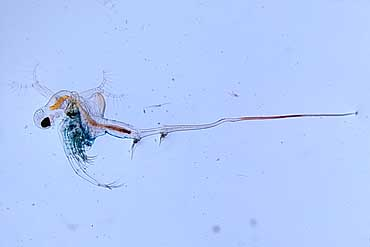
\includegraphics[width=8cm]{waterflea}
\end{center}
\vspace{0.5cm}
\footnotesize{Wisconsin Department of Natural Resources}
\end{frame}
%%%%%

%%%%%
\begin{frame}
\frametitle{\textit{Bythotrephes longimanus}}
\begin{center}
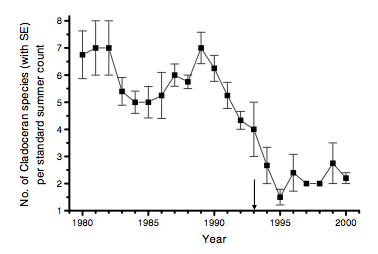
\includegraphics[width=9cm]{Yan}
\end{center}
\vspace{0.5cm}
\footnotesize{Yan et al. (2002)}
\end{frame}
%%%%%

\subsection{Statistical issues}
\frame{\tableofcontents[currentsection,currentsubsection]}

\begin{frame}
\frametitle{Fourth-corner}
\small
% latex table generated in R 2.10.1 by xtable 1.5-6 package
% Tue Feb  8 08:19:58 2011
\begin{table}[ht]
\begin{center}
\begin{tabular}{r|rrrr|r|}
  & sp 1 & sp 2 & sp 3 & sp 4 \\ 
  \hline
site 1 & 0.1 & 2.1 & 0.1 & 1.5  \\ 
  site 2 & 0.7 & -0.9 & 1.8 & 3.7  \\ 
  site 3 & 1.1 & 0.5 & 1.5 & 2.8  \\ 
  site 4 & 1.3 & -2.0 & 3.0 & -0.2  \\ 
  site 5 & 1.7 & 2.0 & 1.3 & 1.2  \\ 
  site 6 & 0.8 & -0.1 & 2.0 & 1.1  \\ 
  site 7 & -2.6 & -1.4 & 1.8 & 4.1  \\ 
  site 8 & -0.0 & 1.5 & 2.3 & 2.3  \\ 
   \hline
\end{tabular}
\end{center}
\end{table}\normalsize
\end{frame}

\begin{frame}
\frametitle{Fourth-corner}
\small
% latex table generated in R 2.10.1 by xtable 1.5-6 package
% Tue Feb  8 08:19:58 2011
\begin{table}[ht]
\begin{center}
\begin{tabular}{r|rrrr|r|}
  & sp 1 & sp 2 & sp 3 & sp 4 & environment \\ 
  \hline
site 1 & 0.1 & 2.1 & 0.1 & 1.5 & -0.3 \\ 
  site 2 & 0.7 & -0.9 & 1.8 & 3.7 & 1.4 \\ 
  site 3 & 1.1 & 0.5 & 1.5 & 2.8 & -0.1 \\ 
  site 4 & 1.3 & -2.0 & 3.0 & -0.2 & 0.4 \\ 
  site 5 & 1.7 & 2.0 & 1.3 & 1.2 & -0.3 \\ 
  site 6 & 0.8 & -0.1 & 2.0 & 1.1 & -0.6 \\ 
  site 7 & -2.6 & -1.4 & 1.8 & 4.1 & 2.0 \\ 
  site 8 & -0.0 & 1.5 & 2.3 & 2.3 & 0.7 \\ 
   \hline
\end{tabular}
\end{center}
\end{table}\normalsize
\end{frame}

\begin{frame}
\frametitle{Fourth-corner}
\small
% latex table generated in R 2.10.1 by xtable 1.5-6 package
% Tue Feb  8 08:19:58 2011
\begin{table}[ht]
\begin{center}
\begin{tabular}{r|rrrr|r|}
  & sp 1 & sp 2 & sp 3 & sp 4 & environment \\ 
  \hline
site 1 & 0.1 & 2.1 & 0.1 & 1.5 & -0.3 \\ 
  site 2 & 0.7 & -0.9 & 1.8 & 3.7 & 1.4 \\ 
  site 3 & 1.1 & 0.5 & 1.5 & 2.8 & -0.1 \\ 
  site 4 & 1.3 & -2.0 & 3.0 & -0.2 & 0.4 \\ 
  site 5 & 1.7 & 2.0 & 1.3 & 1.2 & -0.3 \\ 
  site 6 & 0.8 & -0.1 & 2.0 & 1.1 & -0.6 \\ 
  site 7 & -2.6 & -1.4 & 1.8 & 4.1 & 2.0 \\ 
  site 8 & -0.0 & 1.5 & 2.3 & 2.3 & 0.7 \\ 
   \hline
  trait & -1.0 & -1.0 & 1.0 & 1.0 &  \\ 
   \hline
\end{tabular}
\end{center}
\end{table}\normalsize 
\end{frame}

\begin{frame}
\frametitle{Fourth-corner}
\small
% latex table generated in R 2.10.1 by xtable 1.5-6 package
% Tue Feb  8 08:19:58 2011
\begin{table}[ht]
\begin{center}
\begin{tabular}{r|rrrr|r|}
  & sp 1 & sp 2 & sp 3 & sp 4 & environment \\ 
  \hline
site 1 & 0.1 & 2.1 & 0.1 & 1.5 & -0.3 \\ 
  site 2 & 0.7 & -0.9 & 1.8 & 3.7 & 1.4 \\ 
  site 3 & 1.1 & 0.5 & 1.5 & 2.8 & -0.1 \\ 
  site 4 & 1.3 & -2.0 & 3.0 & -0.2 & 0.4 \\ 
  site 5 & 1.7 & 2.0 & 1.3 & 1.2 & -0.3 \\ 
  site 6 & 0.8 & -0.1 & 2.0 & 1.1 & -0.6 \\ 
  site 7 & -2.6 & -1.4 & 1.8 & 4.1 & 2.0 \\ 
  site 8 & -0.0 & 1.5 & 2.3 & 2.3 & 0.7 \\ 
   \hline
  trait & -1.0 & -1.0 & 1.0 & 1.0 & \textcolor{red}{\textbf{??}} \\ 
   \hline
\end{tabular}
\end{center}
\end{table}\normalsize 
\begin{textblock}{100}(10.2,-0.5)
\textcolor{red}{$\mathbf{\uparrow}$}
\end{textblock}
\begin{textblock}{100}(11,-1.25)
\textcolor{red}{$\mathbf{\leftarrow}$}
\end{textblock}
\begin{textblock}{100}(9.3,-1.25)
\textcolor{red}{$\mathbf{\rightarrow}$}
\end{textblock}
\end{frame}

\begin{frame}
\frametitle{Statistical methods for analyzing `fourth-corner'-esque data}
\begin{center}
\begin{itemize}
\item Chessel et al. (1996) --- RLQ analysis
\item Legendre et al. (1997) --- coined term `fourth-corner'
\item Ives and Godfray (2006) --- mixed models of phylogenetically-structured foodwebs
\item Dray and Legendre (2008) --- extends Legendre et al.
\item Pillar and Duarte (2010) --- phylogenetic null models
\item Leibold et al. (2010) --- semi-partial correlations
\item Ives and Helmus (in press) --- phylogenetic generalized linear mixed models (PGLMMs)
\end{itemize}
\end{center}
\end{frame}

\begin{frame}
\frametitle{The data frame --- replicates-by-variables}
\begin{center}
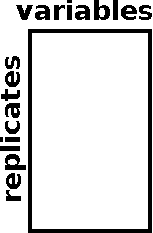
\includegraphics[width=4cm]{dataframe}
\end{center}
\end{frame}

\begin{frame}
\begin{center}
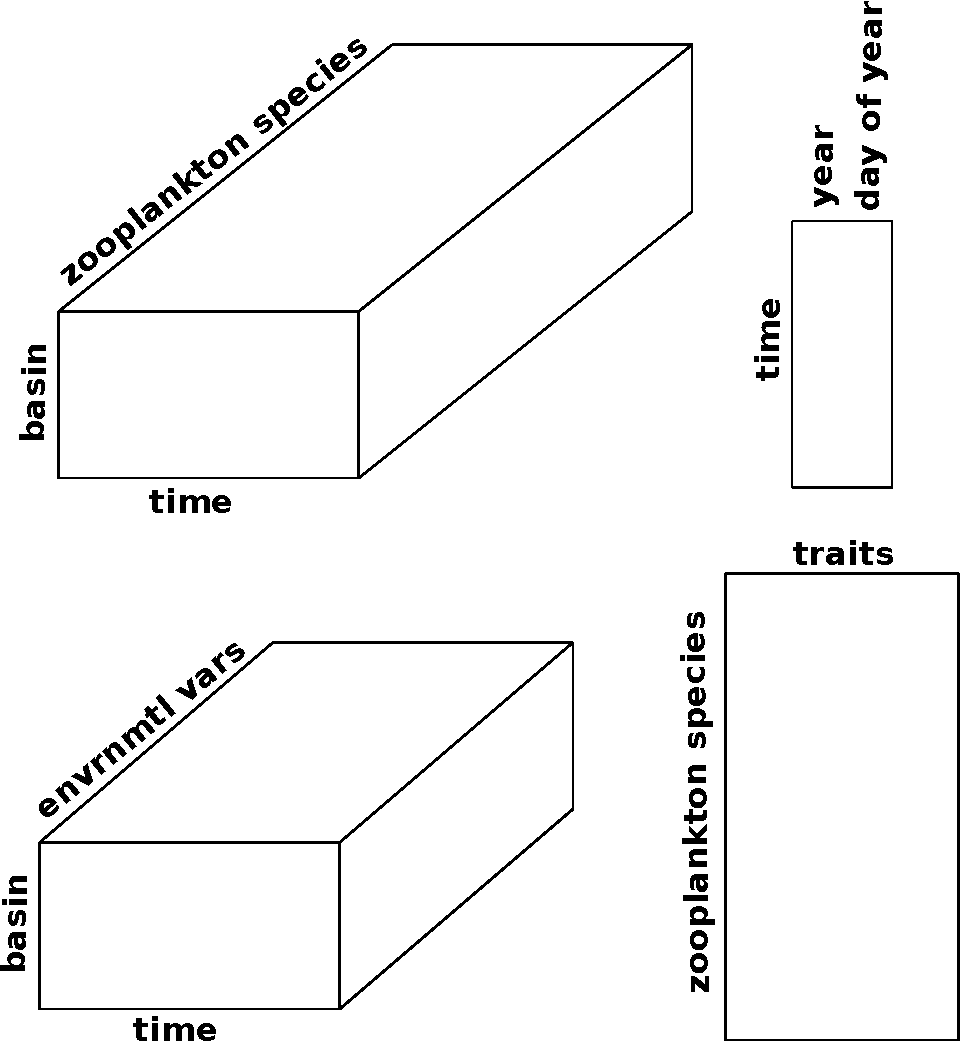
\includegraphics[width=6.5cm]{BeatrixTableCartoon}
\end{center}
\flushleft{Cantin et al. 2011 -- Lac Croche, Qu\'{e}bec, Canada}
\end{frame}

\subsection[Data management]{The data management-analysis interface}
\frame{\tableofcontents[currentsection,currentsubsection]}

\begin{comment}

\begin{frame}
\frametitle{Linear algebra as data management}
\begin{center}
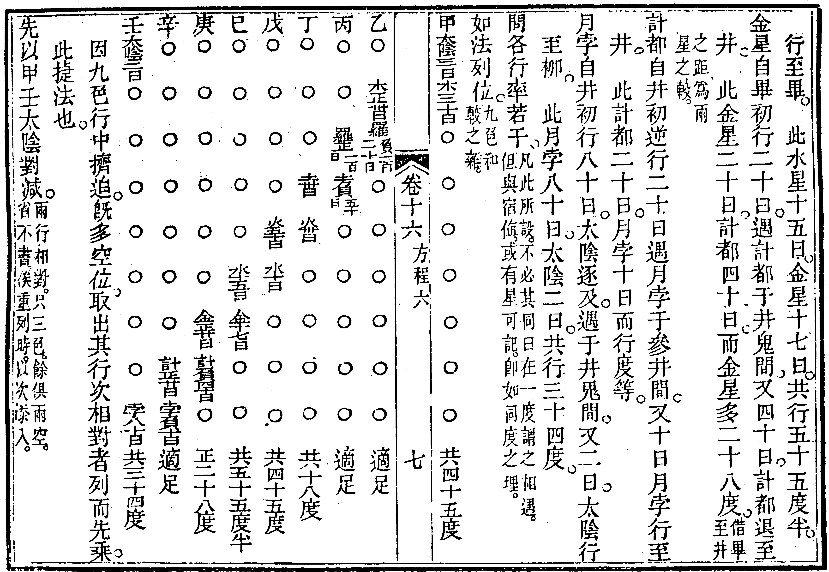
\includegraphics[width=9cm]{fangcheng}
\end{center}
%\vspace{0.5cm}
\footnotesize{Ancient Chinese text ($\sim$150 BCE)}
\end{frame}

\begin{frame}
\frametitle{Linear algebra as data management}
\begin{center}
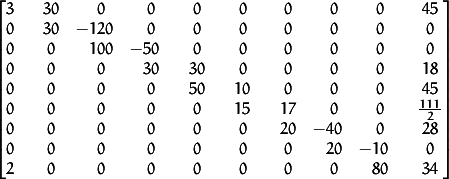
\includegraphics[width=9cm]{fangchengmodern}
\end{center}
%\vspace{0.5cm}
\footnotesize{Hart (2009)}
\end{frame}

\begin{frame}
\frametitle{Linear algebra as data management}
\begin{center}
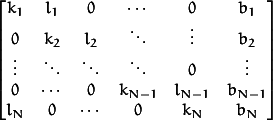
\includegraphics[width=8cm]{fangchengmoderngeneral}
\end{center}
%\vspace{0.5cm}
\footnotesize{Hart (2009)}
\end{frame}

\begin{frame}
\frametitle{Linear algebra as data management}
\begin{center}
\begin{equation}
\begin{split}
\uncover<1->{\mathbf{Y} &= \mathbf{XB}} \\
\uncover<2->{\mathbf{X^{T}Y} &= \mathbf{X^{T}XB}} \\
\uncover<3->{\mathbf{(X^{T}X)}^{-1}\mathbf{X^{T}Y} &= \mathbf{B}} \\
\end{split}
\end{equation}
\end{center}
\uncover<4->{
$\mathbf{Y}$:  a matrix of average species abundances \\
$\mathbf{X}$:  a matrix of environmental variables \\
$\mathbf{B}$:  a matrix of coefficients \\
}
\end{frame}

\begin{frame}
\begin{center}
\begin{block}{The importance of data management to science}
\begin{itemize}
\item Good theories of data management \pause(e.g. matrix algebra) \pause allow us to think at a higher level of abstraction, \pause thereby allowing us to focus on the \emph{interesting new} parts of the problem \pause (e.g. the meaning of $\mathbf{Y,X,B}$). \pause
\item This is because the \emph{uninteresting old} details \pause (e.g. how to solve the linear equation) \pause are automatically correct if the theory is correctly applied \pause (e.g. because it has been previously learned). \pause
\item Therefore, we don't need to actively think about such details \pause \emph{until we step outside of the domain of the theory}.
\end{itemize}
\end{block}
\end{center}
\end{frame}

\end{comment}

\begin{frame}
\frametitle{Linear algebra as data management}
\begin{center}
\begin{block}{Solve for the $b$'s}
\begin{equation}
\begin{array}{ccccccccc}
y_1 & = & b_1 x_{11} & + & b_2 x_{12} & + & \dots & + & b_m x_{1m} \\
y_2 & = & b_ 1 x_{21} & + & b_2 x_{22} & + & \dots & + & b_m x_{2m} \\
\vdots &  & \vdots &  & \vdots &  & \ddots &  & \vdots \\
y_n & = & b_1 x_{n1} & + & b_2 x_{n2} & + & \dots & + & b_m x_{nm} \\
\end{array}
\end{equation}
\end{block}
\end{center}
\end{frame}

\begin{frame}
\frametitle{Linear algebra as data management}
\begin{center}

\uncover<1->{$
\mathbf{y} = \left[
\begin{array}{c}
y_1 \\
y_2 \\
\vdots \\
y_n
\end{array}
\right], \mathbf{X} = \left[
\begin{array}{cccc}
x_{11} & x_{12} & \dots & x_{1m} \\
x_{21} & x_{22} & \dots & x_{2m} \\
\vdots & \vdots & \ddots & \vdots \\
x_{n1} & x_{n2} & \dots & x_{nm} \\
\end{array}
\right], \mathbf{b} = \left[
\begin{array}{c}
b_1 \\
b_2 \\
\vdots \\
b_n
\end{array}
\right]
$}

\begin{equation}
\begin{split}
\uncover<2->{\mathbf{y} &= \mathbf{Xb}} \\
\uncover<3->{\mathbf{X^{T}y} &= \mathbf{X^{T}Xb}} \\
\uncover<3->{\mathbf{(X^{T}X)}^{-1}\mathbf{X^{T}y} &= \mathbf{b}} \\
\end{split}
\end{equation}
\end{center}
\end{frame}

\begin{comment}%%%
\begin{frame}
\frametitle{The R paradigm of data management}
\begin{center}
\vspace{-2cm}
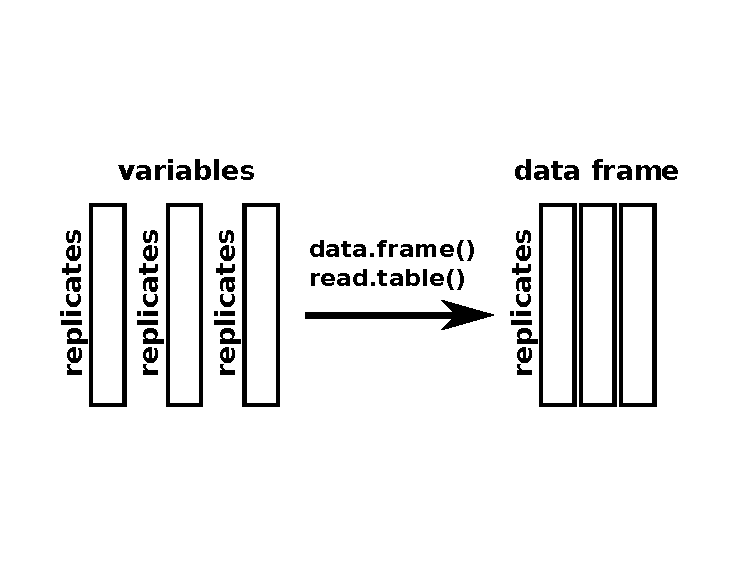
\includegraphics[width=10cm]{vectors2dataframe}
\end{center}
\end{frame}
\end{comment}%%%

\begin{frame}
\frametitle{The R framework for data management}
\begin{center}
\vspace{-1cm}
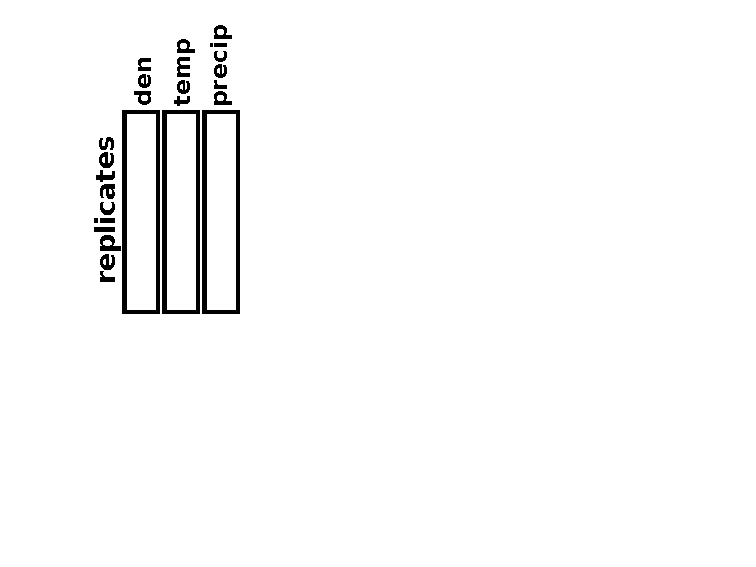
\includegraphics[width=9cm]{dataframe2function1}
\end{center}
\end{frame}

\begin{frame}
\frametitle{The R framework for data management}
\begin{center}
\vspace{-1cm}
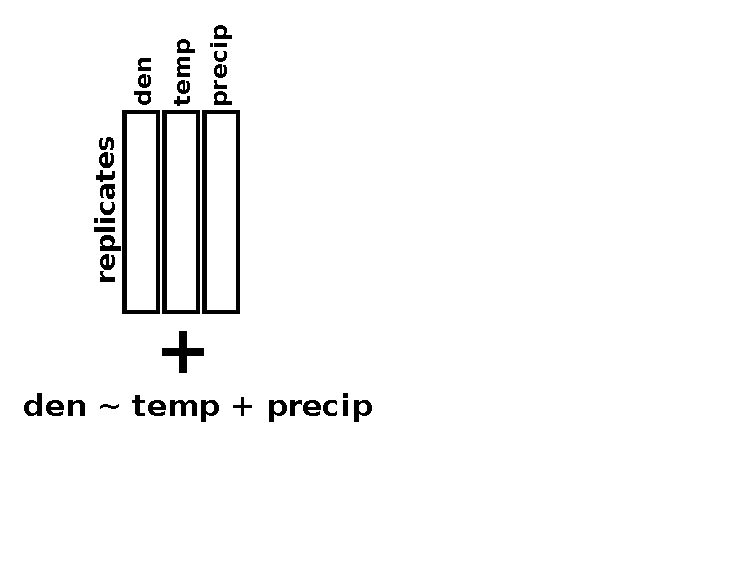
\includegraphics[width=9cm]{dataframe2function2}
\end{center}
\end{frame}

\begin{frame}
\frametitle{The R framework for data management}
\begin{center}
\vspace{-1cm}
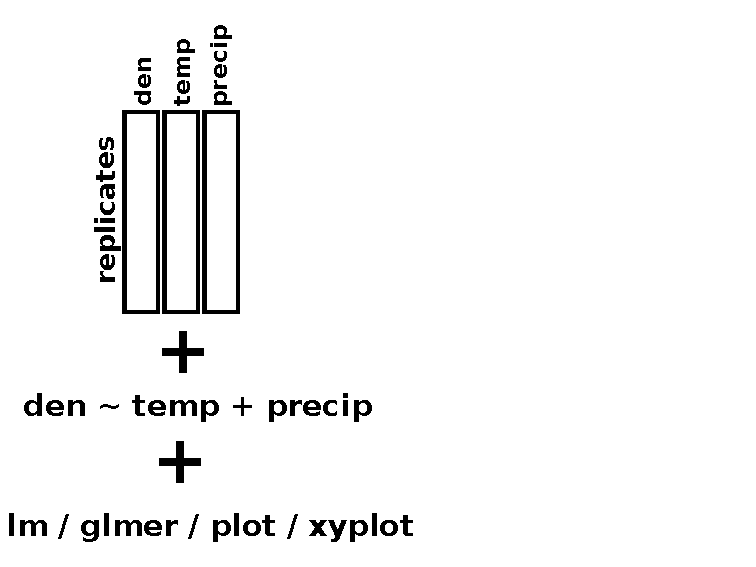
\includegraphics[width=9cm]{dataframe2function3}
\end{center}
\end{frame}

\begin{frame}
\frametitle{The R framework for data management}
\begin{center}
\vspace{-1cm}
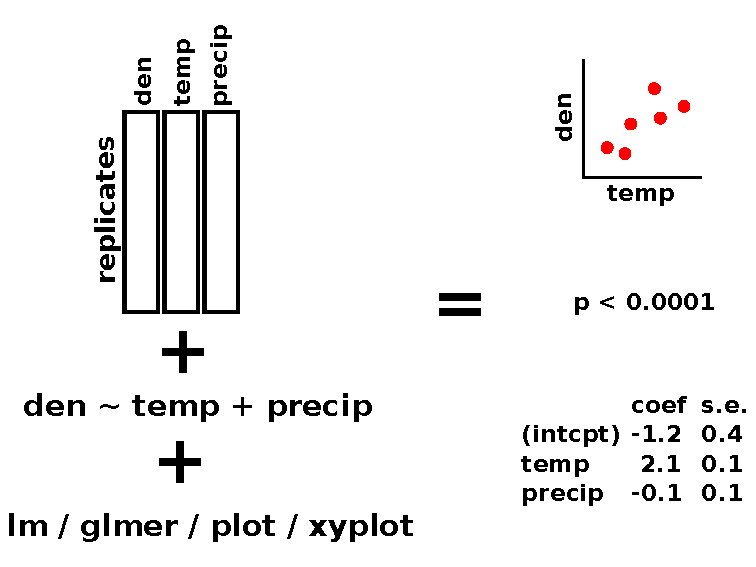
\includegraphics[width=9cm]{dataframe2function4}
\end{center}
\end{frame}

%\begin{small}
\begin{frame}
\frametitle{The R framework for data management}
\begin{center}
\vspace{-0.5cm}
\begin{block}{}
\begin{itemize}
\item This framework allows ecologists to concentrate on their primary interests \pause --- the relationships between ecological variables --- \pause without explicit reference to complex mathematical and algorithmic details.
\pause
\item It also provides access to those details, \pause which are required (1) \pause for more effective analyses and (2) \pause to develop new methods of analysis within the framework.
\pause
\item As new methods are developed, \pause researchers simply pass their data frames to new functions in much the same way they would pass them to older functions.
\pause
\item Thus, by separating low-level methods development from high-level data analysis, \pause \emph{R fosters the formation of a community of researchers where both methodologists and analysts can have mutually beneficial interactions}.
\end{itemize}
\end{block}
\end{center}
\end{frame}
%\end{small}

\begin{comment}%%%
\setlength{\tabcolsep}{2.5pt}
\begin{frame}
\frametitle{The R paradigm of data management}
\begin{center}
\begin{tabular}{ccccccc}
DATA FRAME&+&FORMULA&+&FUNCTION&=&ANALYSIS \\
\\
\end{tabular}
\end{center}
\end{frame}
\setlength{\tabcolsep}{6pt}

\setlength{\tabcolsep}{2.5pt}
\begin{frame}
\frametitle{The R paradigm of data management}
\begin{center}
\begin{tabular}{ccccccc}
\textbf{DATA FRAME}&+&FORMULA&+&FUNCTION&=&ANALYSIS \\
data management \\
\end{tabular}
\end{center}
\end{frame}
\setlength{\tabcolsep}{6pt}

\setlength{\tabcolsep}{2.5pt}
\begin{frame}
\frametitle{The R paradigm of data management}
\begin{center}
\begin{tabular}{ccccccc}
DATA FRAME&+&\textbf{FORMULA}&+&FUNCTION&=&ANALYSIS \\
&&ecological ideas \\
\end{tabular}
\end{center}
\end{frame}
\setlength{\tabcolsep}{6pt}

\setlength{\tabcolsep}{2.5pt}
\begin{frame}
\frametitle{The R paradigm of data management}
\begin{center}
\begin{tabular}{ccccccc}
DATA FRAME&+&FORMULA&+&\textbf{FUNCTION}&=&ANALYSIS \\
&&&&algorithms \\
\end{tabular}
\end{center}
\end{frame}
\setlength{\tabcolsep}{6pt}

\setlength{\tabcolsep}{2.5pt}
\begin{frame}
\frametitle{The R paradigm of data management}
\begin{center}
\begin{tabular}{ccccccc}
DATA FRAME&+&FORMULA&+&FUNCTION&=&\textbf{ANALYSIS} \\
 \\
\end{tabular}
\end{center}
\end{frame}
\setlength{\tabcolsep}{6pt}
\end{comment}%%%

\setlength{\tabcolsep}{2.5pt}
\begin{frame}
\begin{block}{}
\begin{description}
\item[Goal] \uncover<1->{Analyze multiple table data sets using this framework}
\item[Problem] \uncover<2->{R doesn't do multiple tables `out-of-the-box'}
\item[Strategy] \uncover<3->{Develop some theory to better understand multiple table data management and then use that theory to extend the R framework to allow multiple table data sets}
\end{description}
\end{block}
\begin{center}
\begin{tabular}{ccccccc}
\uncover<5->{DATA LIST \\
$\downarrow$} \\
\uncover<4->{DATA FRAME&+&FORMULA&+&FUNCTION&=&ANALYSIS} \\
\\
\end{tabular}
\end{center}
\end{frame}
\setlength{\tabcolsep}{6pt}

\section{Theory}
\subsection[Multiple $\to$ single]{Converting multiple tables to one single table}
\frame{\tableofcontents[currentsection,currentsubsection]}

\begin{comment}
\begin{frame}
\frametitle{The data frame --- replicates-by-variables}
\begin{center}
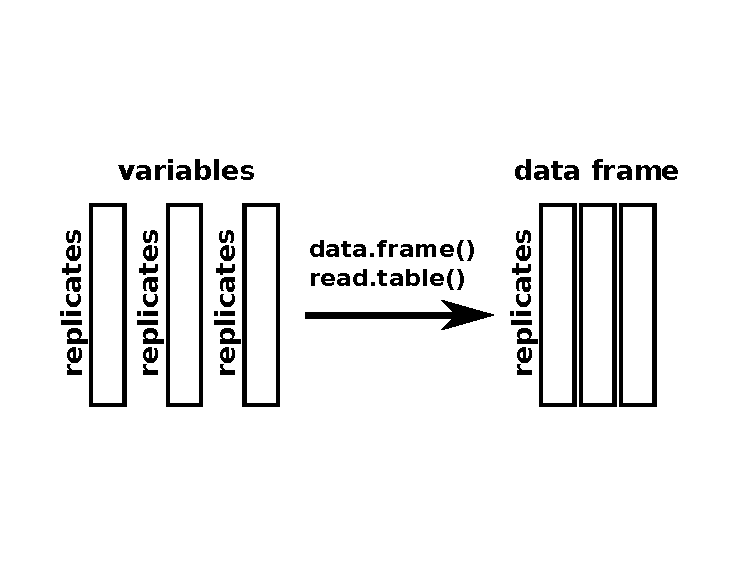
\includegraphics[width=10cm]{vectors2dataframe}
\end{center}
\end{frame}
\end{comment}

\begin{frame}
\frametitle{How can we convert this to a data frame?}
\begin{center}
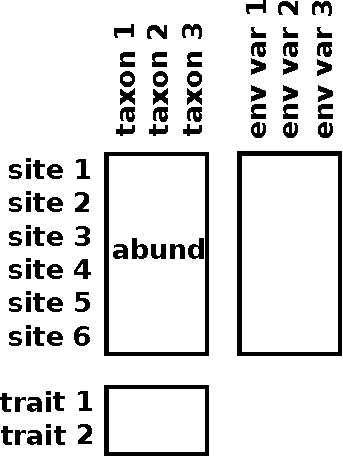
\includegraphics[width=3.7cm]{forthcorner}
\pause
\begin{textblock}{4}(0,-10.6)
\begin{block}{}
\begin{itemize}
\item Lost information
\item Redundant information
\end{itemize}
\end{block}
\end{textblock}
\end{center}
\end{frame}

\begin{comment}%%
\begin{frame}
\frametitle{Drop data}
\begin{center}
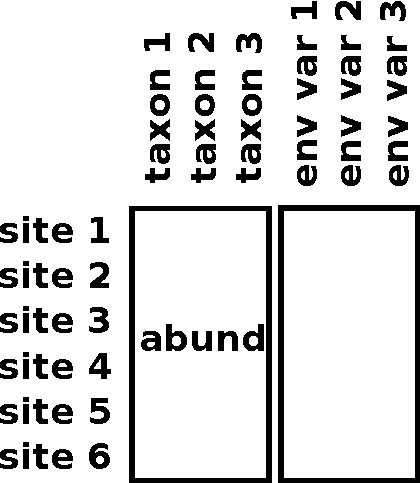
\includegraphics[width=3.7cm]{forthcorner2dataframeDROP}
\end{center}
\end{frame}
\end{comment}%%

\begin{frame}
\frametitle{Lost information}
\begin{center}
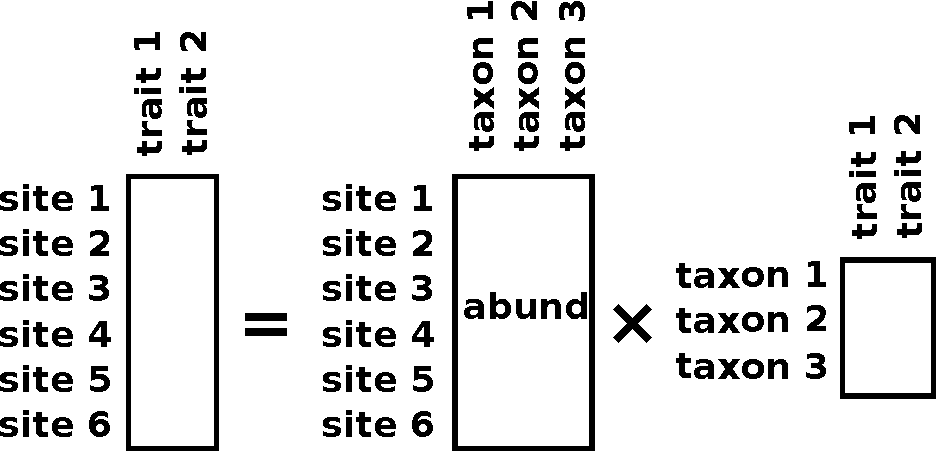
\includegraphics[width=9cm]{forthcorner2dataframeSUMMARIZE1}
\end{center}
\footnotesize{e.g. Leibold et al. (2010)}
\end{frame}

\begin{frame}
\frametitle{Lost information}
\begin{center}
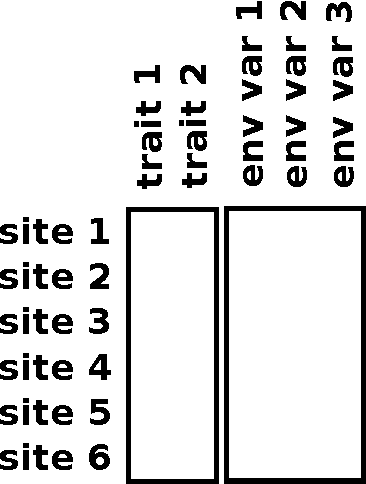
\includegraphics[width=4cm]{forthcorner2dataframeSUMMARIZE2}
\end{center}
\footnotesize{e.g. Leibold et al. (2010)}
\end{frame}

\begin{frame}
\frametitle{Redundant information}
\begin{center}
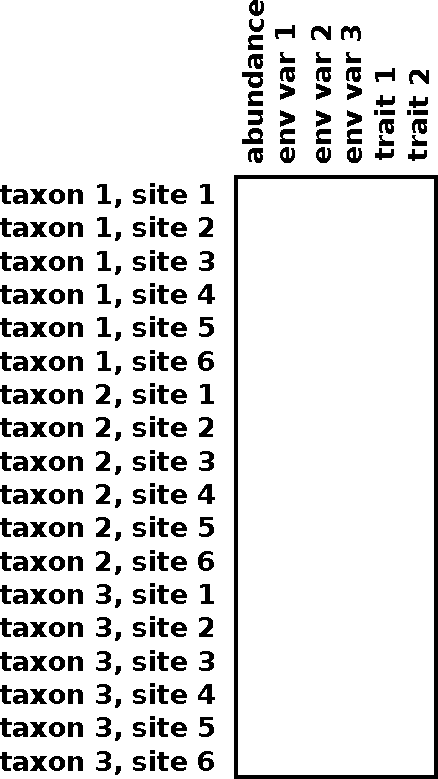
\includegraphics[width=4cm]{forthcorner2dataframeREPEAT}
\end{center}
\end{frame}

\begin{frame}
\frametitle{Redundant information}
\begin{center}
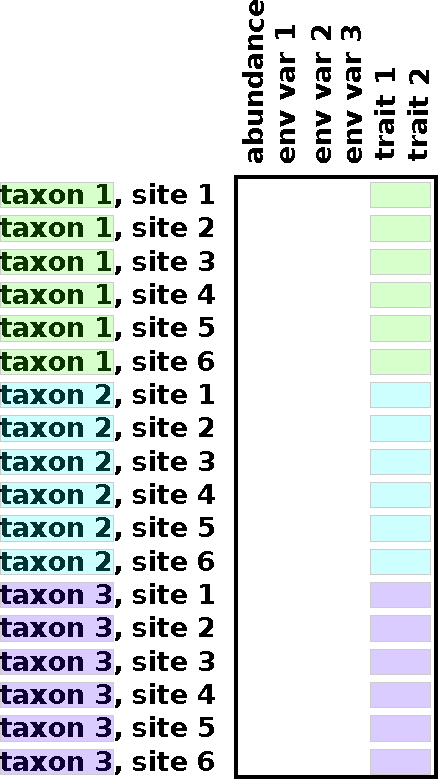
\includegraphics[width=4cm]{forthcorner2dataframeREPEAT3}
\end{center}
\end{frame}

\begin{frame}
\frametitle{Redundant information}
\begin{center}
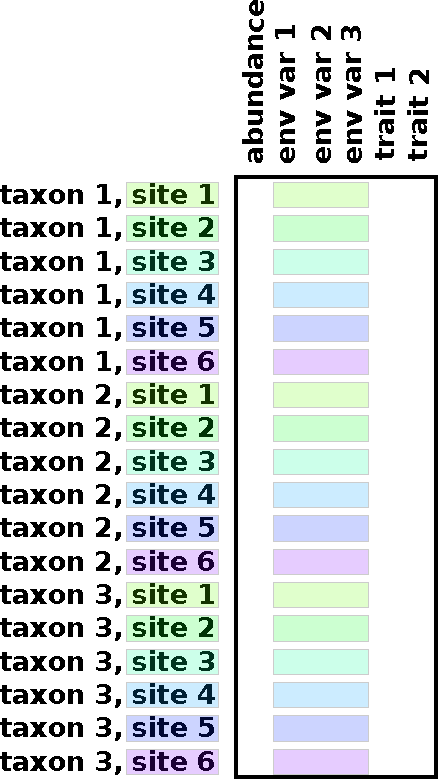
\includegraphics[width=4cm]{forthcorner2dataframeREPEAT2}
\end{center}
\end{frame}

\begin{frame}
\frametitle{Redundant information}
\begin{center}
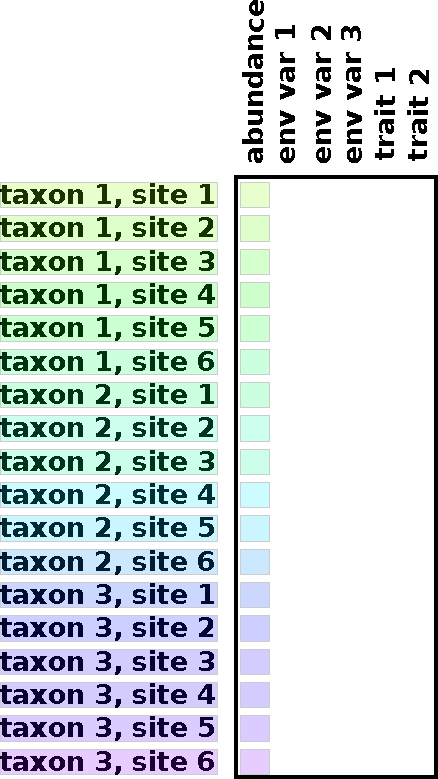
\includegraphics[width=4cm]{forthcorner2dataframeREPEAT1}
\end{center}
\end{frame}

\begin{comment}%%%
\begin{frame}
\frametitle{The data frame --- replicates-by-variables}
\begin{center}
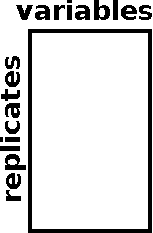
\includegraphics[width=4cm]{dataframe}
\end{center}
\end{frame}
\end{comment}%%%

\begin{frame}
\frametitle{Classifying the fourth-corner dimensions}
\begin{center}
\begin{block}{Rules}
\begin{itemize}
\item Dimensions that \emph{can not grow} with more sampling represent \emph{groups of variables}
\pause
\item Dimensions that \emph{can grow} with more sampling represent \emph{replication}
\end{itemize}
\end{block}
\end{center}
\end{frame}

\begin{frame}
\frametitle{Classifying the fourth-corner dimensions}
\begin{center}
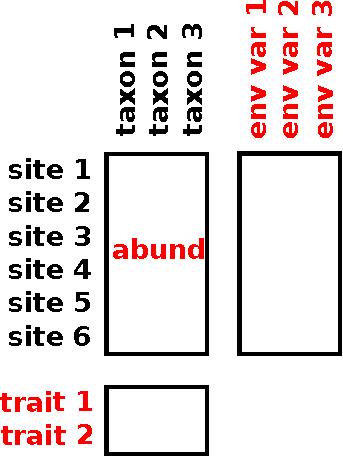
\includegraphics[width=3.8cm]{forthcornerVARIABLES}
\begin{textblock}{4}(0,-10.9)
\begin{block}{Variables}
\begin{itemize}
\item \textcolor{red}{abundance}
\item \textcolor{red}{environmental variables}
\item \textcolor{red}{traits}
\end{itemize}
\end{block}
\end{textblock}
\end{center}
\end{frame}

\begin{frame}
\frametitle{Classifying the fourth-corner dimensions}
\begin{center}
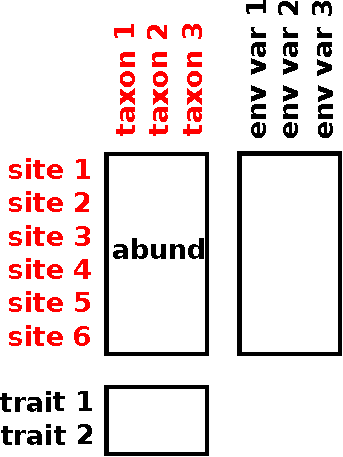
\includegraphics[width=3.8cm]{forthcornerREPLICATES}
\begin{textblock}{4}(0,-10.9)
\begin{block}{Replicates}
\begin{itemize}
\item \textcolor{red}{sites}
\item \textcolor{red}{taxa}
\end{itemize}
\end{block}
\end{textblock}
\end{center}
\end{frame}

\begin{frame}
\frametitle{Classifying the fourth-corner dimensions}
\begin{center}
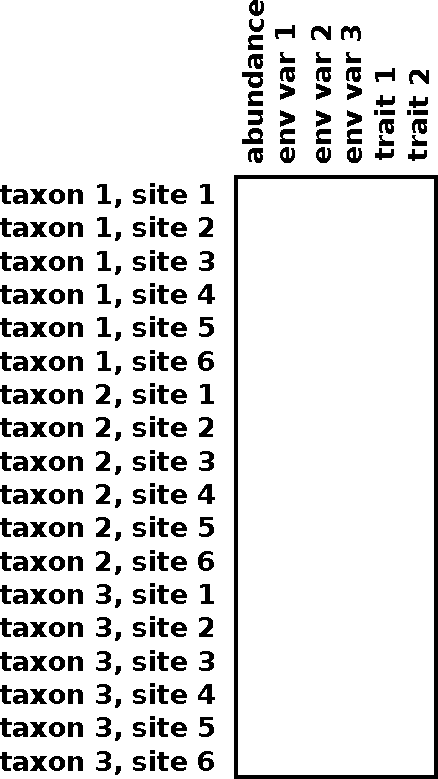
\includegraphics[width=4cm]{forthcorner2dataframeREPEAT}
\end{center}
\end{frame}

\subsection[Bipartite graphs]{Analyzing data structure with bipartite graphs}
\frame{\tableofcontents[currentsection,currentsubsection]}

\begin{frame}
\frametitle{Bipartite graphs}
\begin{center}
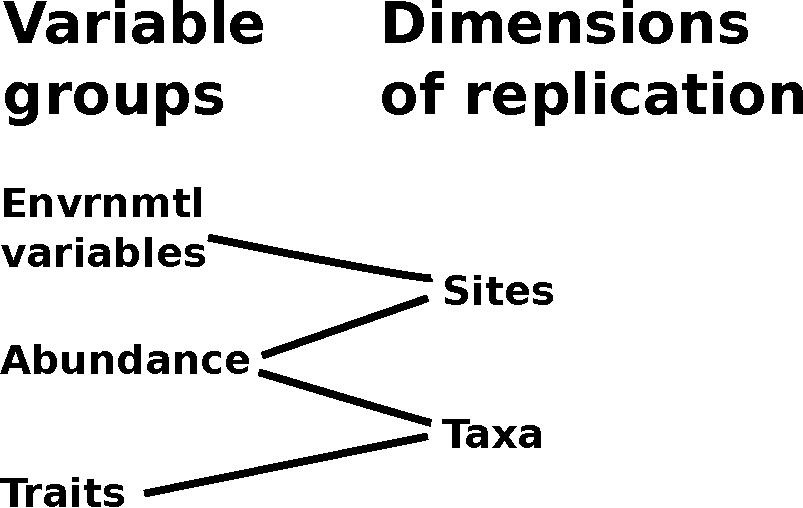
\includegraphics[width=7cm]{bipartiteFC}
\end{center}
\end{frame}

\begin{comment}%%%
\begin{frame}
\frametitle{Bipartite graphs}
\begin{center}
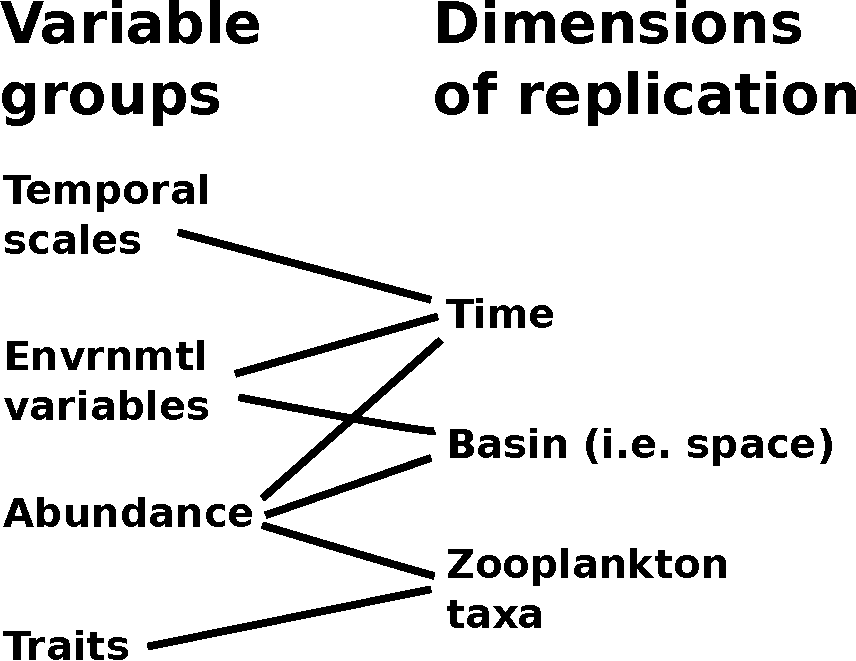
\includegraphics[width=7cm]{bipartiteBEA}
\end{center}
\flushleft{Cantin et al. 2011 -- Lac Croche, Qu\'{e}bec, Canada}
\end{frame}
\end{comment}%%%

\begin{frame}
\frametitle{Biadjacency matrices}
\begin{flushleft}
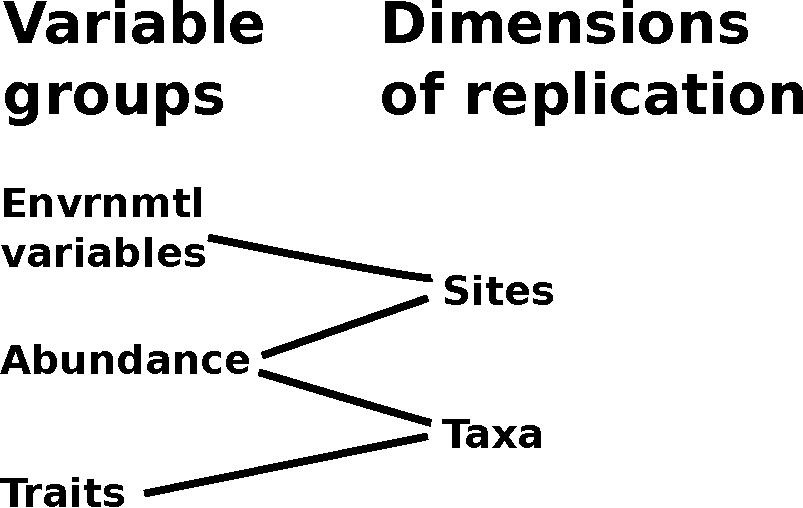
\includegraphics[width=5cm]{bipartiteFC}
\begin{tabular}{cccc}
& abund. & env. & traits \\ 
sites & 1  &  1 & 0 \\
taxa & 1  &  0 & 1 \\
\end{tabular}
\end{flushleft}
\end{frame}

\begin{frame}
\frametitle{Biadjacency matrices}
\begin{block}{Identifying data sets that are not multiple-table}
\uncover<1->{If a data set has a biadjacency matrix with at least one row of all ones,} \uncover<3->{then that data set can be expressed as a single table} \uncover<4->{without redundant or lost information.}
\end{block}
\uncover<2->{
\begin{block}{Example}
\begin{flushleft}
%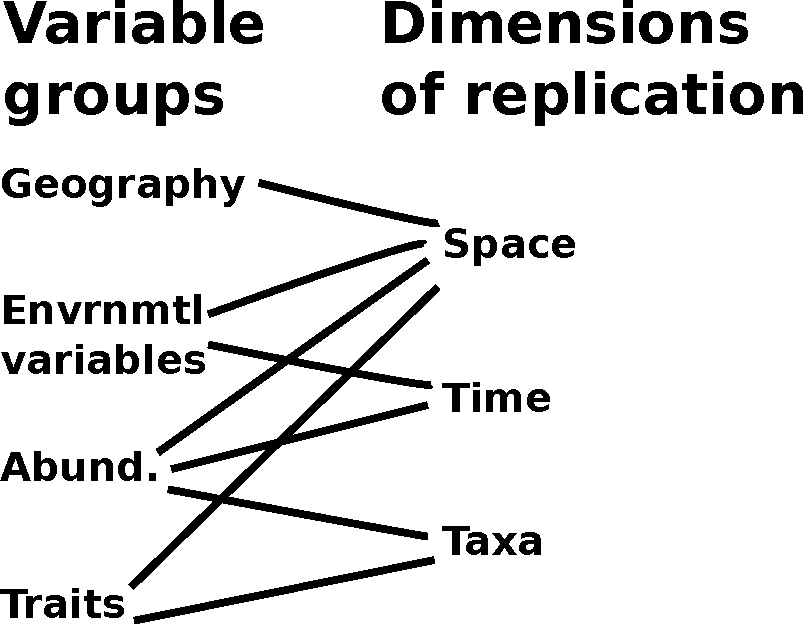
\includegraphics[width=5cm]{bipartiteLEG2}
\begin{tabular}{ccccc}
& abund. & env. & geog. & traits \\ 
space & 1  &  1 & 1 & 1\\
time & 1  &  1 & 0 & 0\\
taxa & 1 & 0 & 0 & 1\\
\end{tabular}
\end{flushleft}
\end{block}
}
\end{frame}

\begin{comment}%%%
\begin{frame}
\frametitle{Biadjacency matrices}
\begin{flushleft}
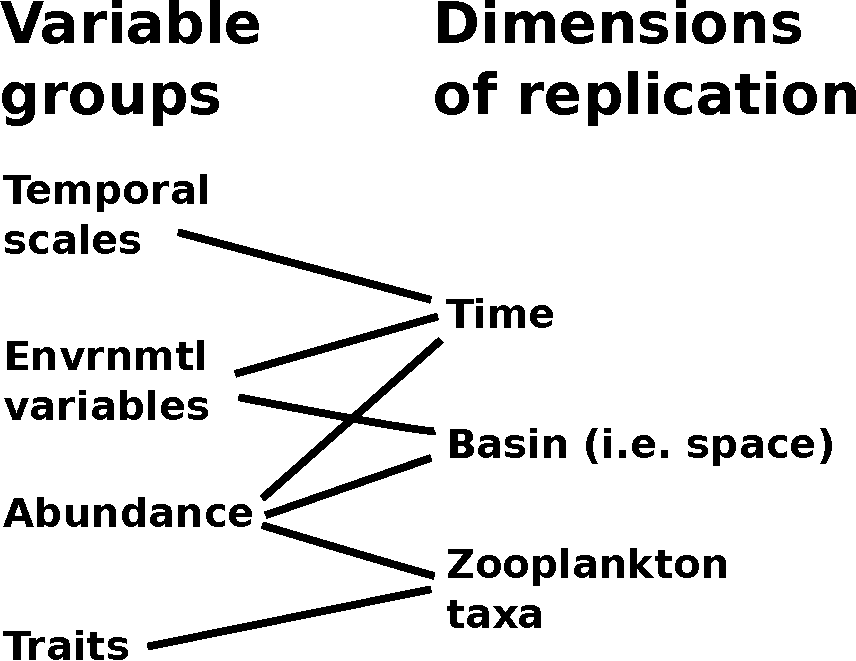
\includegraphics[width=5cm]{bipartiteBEA} \\
\vspace{10pt}
\begin{tabular}{ccccc}
& abund. & env. & temp. & traits \\ 
time & 1  &  1 & 1 & 0\\
basin & 1  &  1 & 0 & 0\\
taxa & 1 & 0 & 0 & 1\\
\end{tabular}
\end{flushleft}
\flushleft{Cantin et al. 2011 -- Lac Croche, Qu\'{e}bec, Canada}
\end{frame}
\end{comment}%%%

\begin{frame}
\frametitle{Biadjacency matrices}
\begin{block}{Necessarily un-correlated variables}
\uncover<1->{If two columns in a biadjacency matrix are orthogonal (i.e. have zero dot product)} \uncover<3->{then the associated variable groups are also orthogonal (i.e. uncorrelated),} \uncover<4->{after the data set has been coerced to a data frame by the method of repetition.}
\end{block}
\uncover<2->{
\begin{block}{Example}
\begin{flushleft}
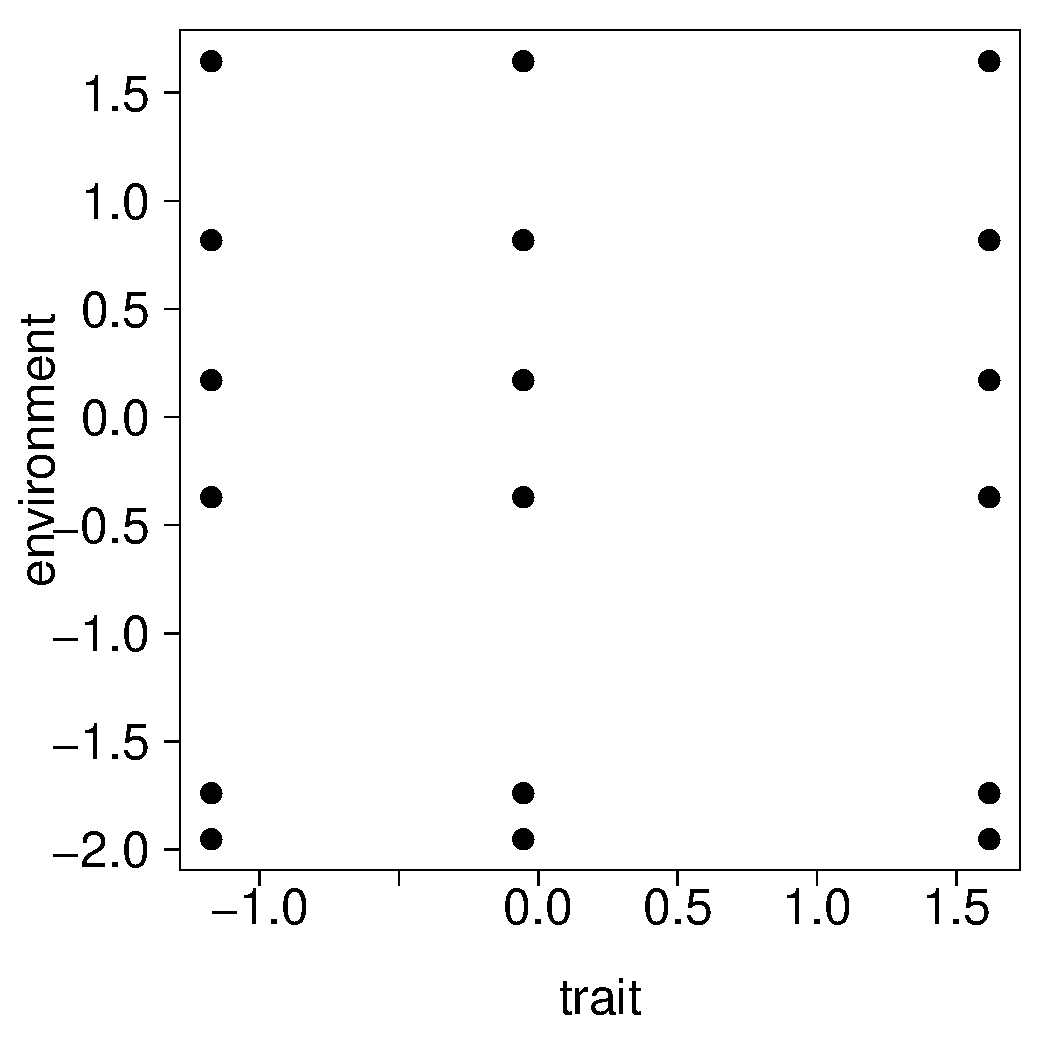
\includegraphics[width=4cm]{uncorr}
\begin{textblock}{4}(5.5,-6)
\begin{tabular}{cccc}
& abund. & env. & traits \\ 
sites & 1  &  1 & 0 \\
taxa & 1  &  0 & 1 \\
\end{tabular}
\end{textblock}
\end{flushleft}
\end{block}
}
\end{frame}

\begin{comment}%%%
\begin{frame}
\frametitle{Biadjacency matrices}
\begin{flushleft}
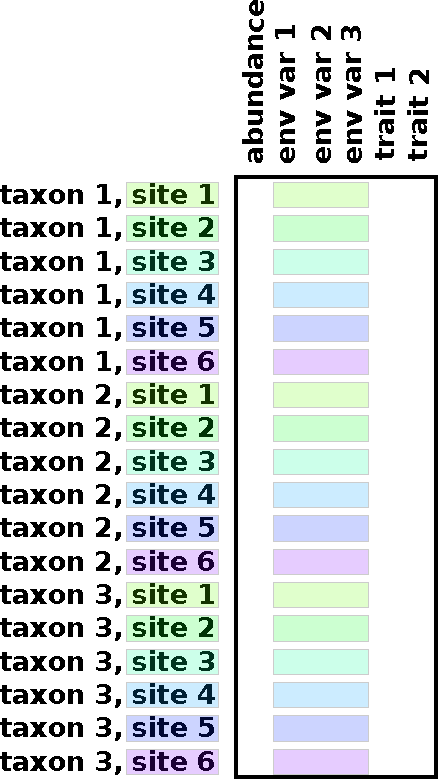
\includegraphics[width=4cm]{forthcorner2dataframeREPEAT2}
\begin{textblock}{10}(6,-7)
\begin{tabular}{cccc}
& abund. & env. & traits \\ 
sites & 1  &  1 & 0 \\
taxa & 1  &  0 & 1 \\
\end{tabular}
\end{textblock}
\end{flushleft}
\end{frame}
\end{comment}%%%

\begin{comment}%%%
\begin{frame}
\frametitle{Biadjacency matrices}
\begin{tabular}{cccc}
& abund. & env. & traits \\ 
sites & 1  &  1 & 0 \\
taxa & 1  &  0 & 1 \\
\end{tabular}
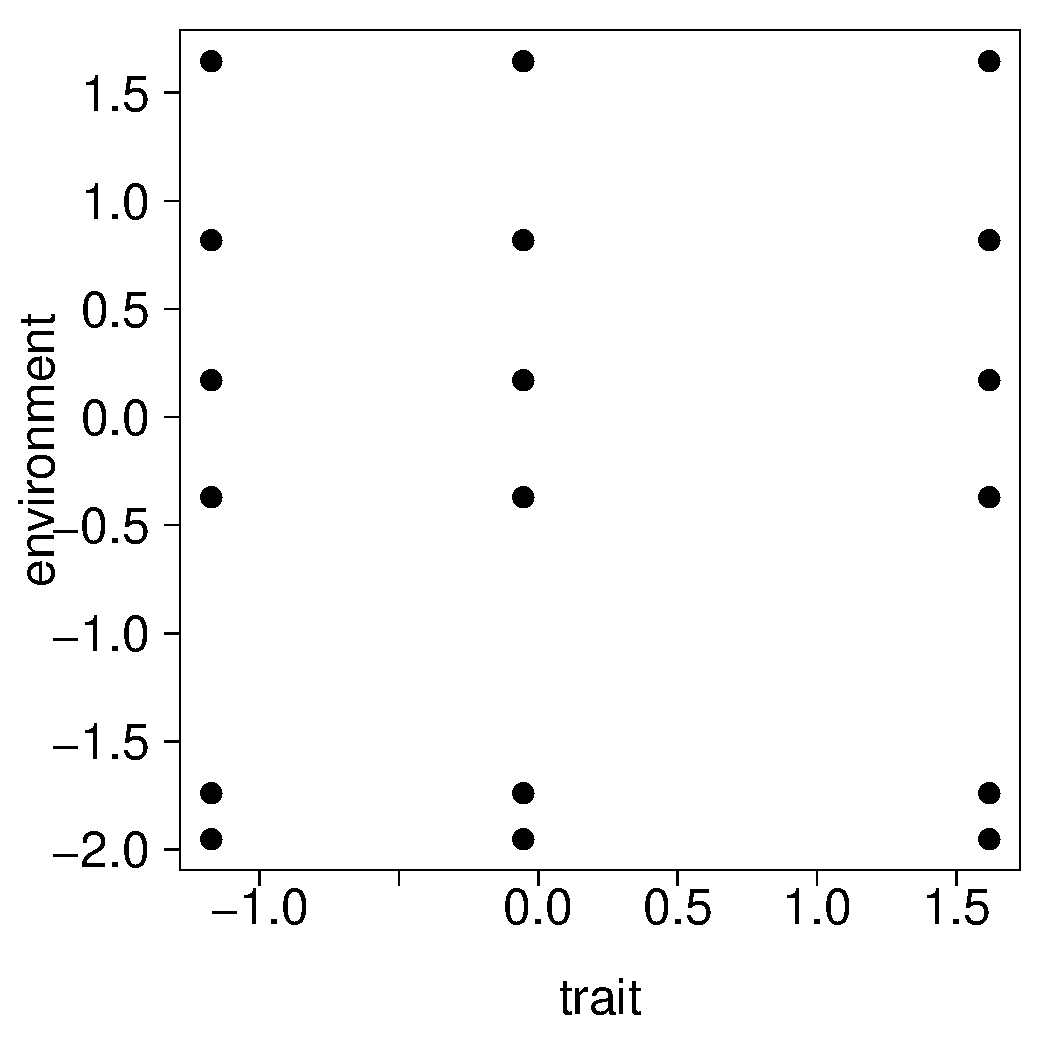
\includegraphics[width=5cm]{uncorr}
\end{frame}
\end{comment}%%%

\begin{comment}%%%
\begin{frame}
\frametitle{Biadjacency matrices}
\begin{flushleft}
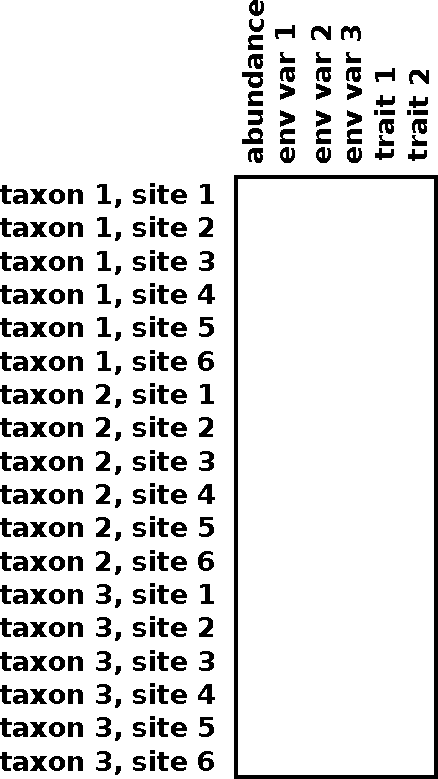
\includegraphics[width=4cm]{forthcorner2dataframeREPEAT}
\begin{textblock}{10}(6,-11)
\begin{tabular}{cccc}
& abund. & env. & traits \\ 
sites & 1  &  1 & 0 \\
taxa & 1  &  0 & 1 \\
\end{tabular}
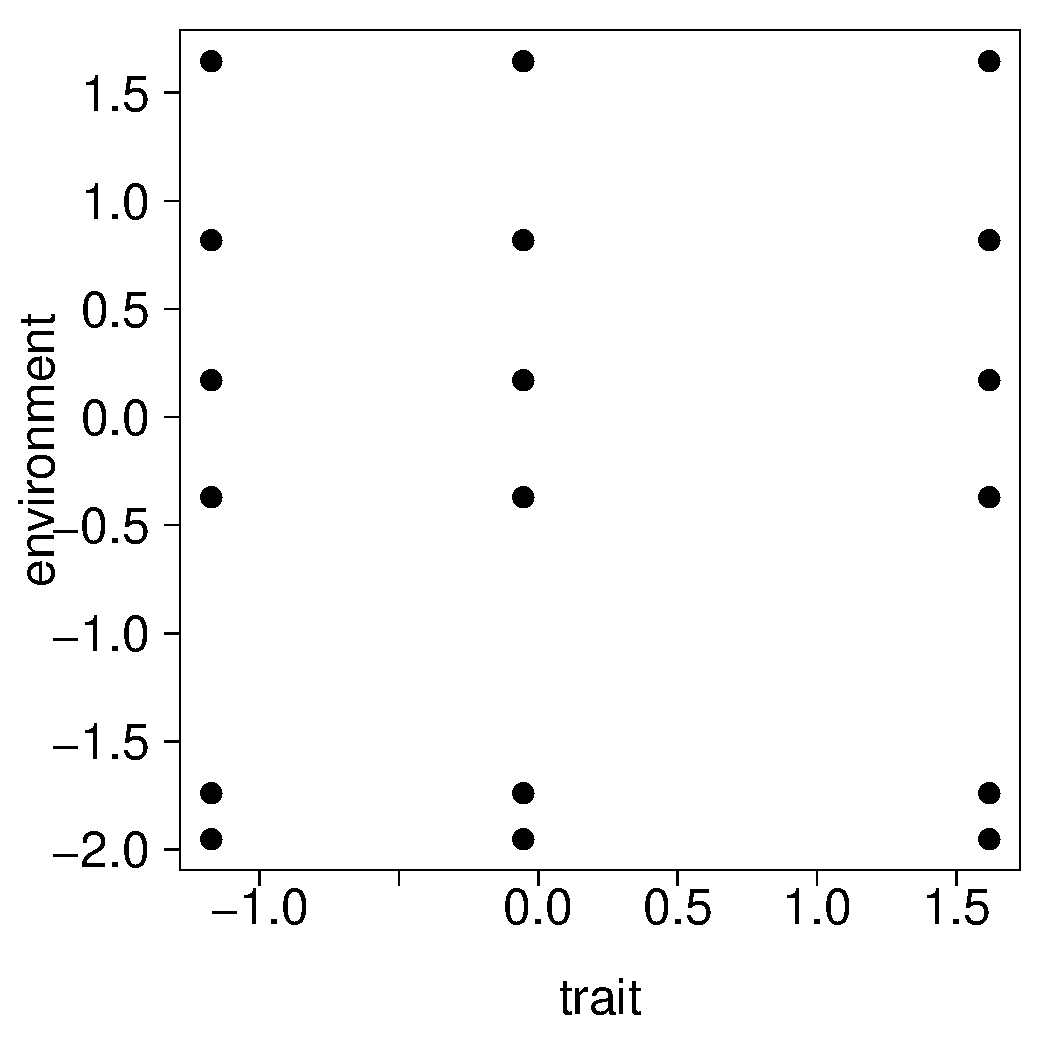
\includegraphics[width=5cm]{uncorr}
\end{textblock}
\end{flushleft}
\end{frame}
\end{comment}%%%

\begin{frame}
\frametitle{Biadjacency matrices}
\begin{center}
\begin{block}{The meaning of zeros}
A variable with a zero for a particular dimension of replication, is assumed (statistically) constant across that dimension.
\end{block}
\pause
\begin{block}{Example}
\begin{tabular}{cccc}
& abund. & env. & traits \\ 
sites & 1  &  1 & 0 \\
taxa & 1  &  0 & 1 \\
\end{tabular}
\end{block}
\end{center}
\end{frame}

\begin{comment}%%%
\begin{frame}
\frametitle{Biadjacency matrices}
\begin{flushleft}
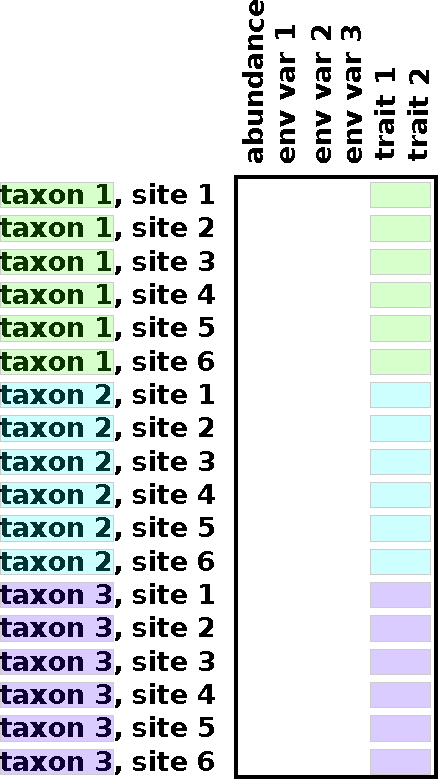
\includegraphics[width=4cm]{forthcorner2dataframeREPEAT3}
\begin{textblock}{10}(6,-11)
\begin{tabular}{cccc}
& abund. & env. & traits \\ 
sites & 1  &  1 & 0 \\
taxa & 1  &  0 & 1 \\
\end{tabular}
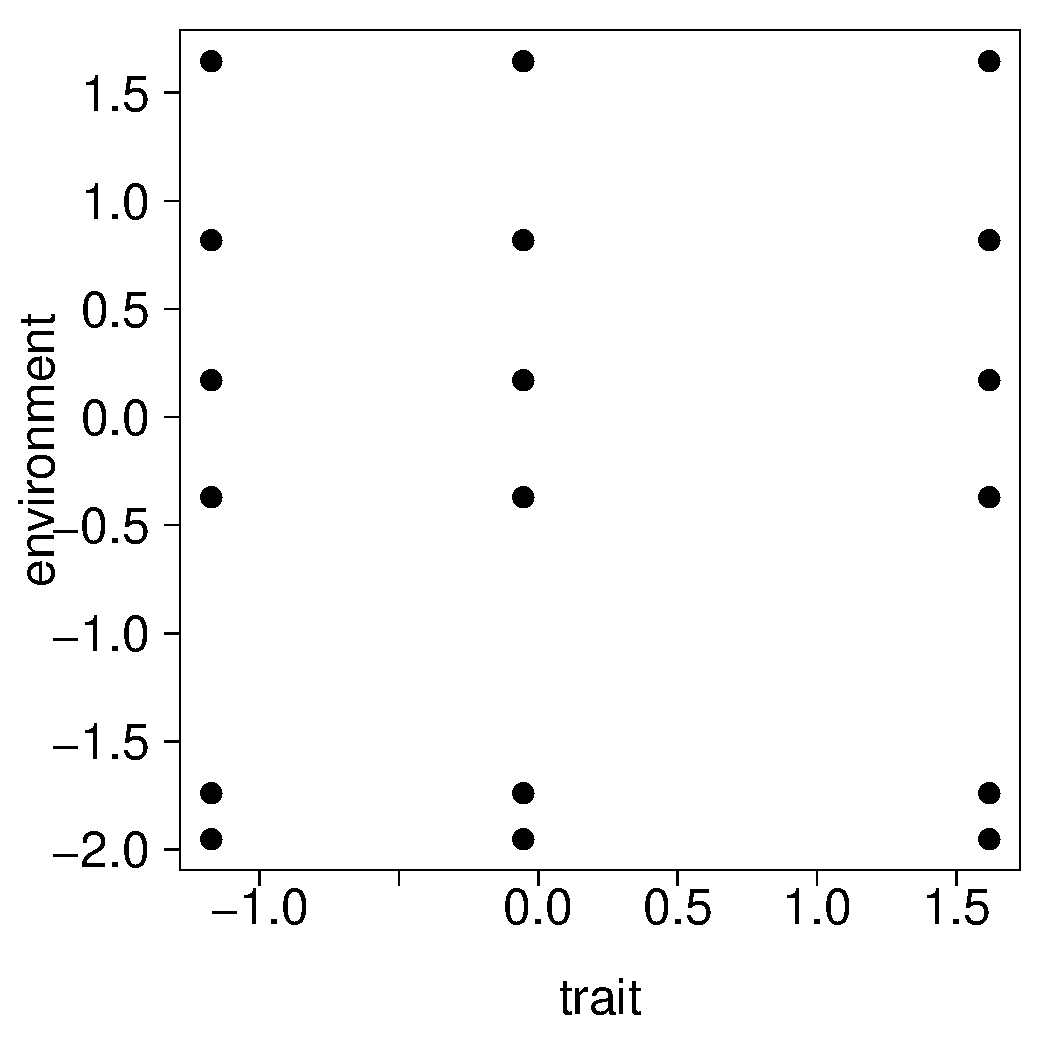
\includegraphics[width=5cm]{uncorr}
\end{textblock}
\end{flushleft}
\end{frame}
\end{comment}%%%

\section[Methods]{Computational methods}

\begin{frame}[fragile]
\begin{Schunk}
\begin{Sinput}
> library(multitable)
\end{Sinput}
\end{Schunk}
http://multitable.r-forge.r-project.org/ \\
\vspace{0.3cm}
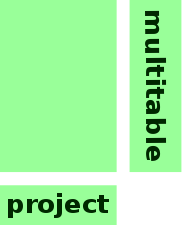
\includegraphics[width=3cm]{multitablelogo} \quad

\includegraphics[width=3cm]{Rforgelogo}
\end{frame}

\subsection[Data lists]{Multiple tables in one R object: the data list}
\frame{\tableofcontents[currentsection,currentsubsection]}

\begin{comment}%%%
\begin{frame}[fragile]
\begin{Schunk}
\begin{Sinput}
> ab
\end{Sinput}
\begin{Soutput}
       sppA  sppB  sppC
siteA  1.17 -0.04  0.85
siteB  0.65 -0.06 -0.37
siteC  0.51 -2.73  1.07
siteD -1.19  2.81  0.17
siteE -0.69 -0.21  0.38
\end{Soutput}
\end{Schunk}
\end{frame}

\begin{frame}[fragile]
\begin{Schunk}
\begin{Sinput}
> tp
\end{Sinput}
\begin{Soutput}
siteA siteB siteC siteD siteE 
-1.04  0.77  0.82 -0.38 -0.06 
\end{Soutput}
\end{Schunk}
\end{frame}

\begin{frame}[fragile]
\begin{Schunk}
\begin{Sinput}
> bs
\end{Sinput}
\begin{Soutput}
 sppA  sppB  sppC 
-0.45 -0.07  1.48 
\end{Soutput}
\end{Schunk}
\end{frame}
\end{comment}%%%

\begin{frame}[fragile]
\begin{Schunk}
\begin{Sinput}
> dl <- data.list(abundance = ab, temperature = tp,
+	bodysize = bs, dnames = c("sites", "species"))
\end{Sinput}
\end{Schunk}
\end{frame}

\begin{frame}[fragile]
\begin{Schunk}
\begin{Soutput}
> dl
abundance:
---------
       sppA  sppB  sppC
siteA  1.17 -0.04  0.85
siteB  0.65 -0.06 -0.37
siteC  0.51 -2.73  1.07
siteD -1.19  2.81  0.17
siteE -0.69 -0.21  0.38
Replicated along:  || sites || || species ||

temperature:
-----------
siteA siteB siteC siteD siteE 
-1.04  0.77  0.82 -0.38 -0.06 
Replicated along:  || sites || 
\end{Soutput}
\end{Schunk}
\begin{block}{}
\flushright{continued...}
\end{block}
\end{frame}

\begin{frame}[fragile]
\begin{Schunk}
\begin{Soutput}
bodysize:
--------
 sppA  sppB  sppC 
-0.45 -0.07  1.48 
Replicated along:  || species || 


REPLICATION DIMENSIONS: 
  sites species 
      5       3 
\end{Soutput}
\end{Schunk}
\end{frame}

\begin{comment}%%
\begin{frame}[fragile]
\begin{Schunk}
\begin{Sinput}
> summary(dl)
\end{Sinput}
\begin{Soutput}
        abundance temperature bodysize
sites        TRUE        TRUE    FALSE
species      TRUE       FALSE     TRUE
\end{Soutput}
\end{Schunk}
\end{frame}

\begin{frame}[fragile]
\begin{Schunk}
\begin{Sinput}
> str(dl)
\end{Sinput}
\begin{Soutput}
List of 3
 $ abundance  : num [1:5, 1:3] 1.17 0.65 0.51...
 $ temperature: num [1:5(1d)] -1.04 0.77 0.82 ...
 $ bodysize   : num [1:3(1d)] -0.45 -0.07 1.48
\end{Soutput}
\end{Schunk}
\end{frame}
\end{comment}

\subsection[Subscripting]{Subscripting multiple tables simultaneously}
\frame{\tableofcontents[currentsection,currentsubsection]}


\begin{frame}[fragile]
\begin{Schunk}
\begin{Sinput}
> dl[1:3, ]
\end{Sinput}
\end{Schunk}
\end{frame}

\begin{frame}[fragile]
\begin{Schunk}
\begin{Soutput}
abundance:
---------
      sppA  sppB  sppC
siteA 1.17 -0.04  0.85
siteB 0.65 -0.06 -0.37
siteC 0.51 -2.73  1.07
Replicated along:  || sites || species || 


temperature:
-----------
siteA siteB siteC 
-1.04  0.77  0.82 
Replicated along:  || sites || 
\end{Soutput}
\end{Schunk}
\begin{block}{}
\flushright{continued...}
\end{block}
\end{frame}

\begin{frame}[fragile]
\begin{Schunk}
\begin{Soutput}
bodysize:
--------
 sppA  sppB  sppC 
-0.45 -0.07  1.48 
Replicated along:  || species || 


REPLICATION DIMENSIONS: 
  sites species 
      3       3 
\end{Soutput}
\end{Schunk}
\end{frame}

\begin{comment}%%%
\begin{frame}[fragile]
\begin{Schunk}
\begin{Sinput}
> dl[, "sppB"]
\end{Sinput}
\begin{Soutput}
abundance:
---------
       sppB
siteA -0.04
siteB -0.06
siteC -2.73
siteD  2.81
siteE -0.21
Replicated along:  || sites || species || 


temperature:
-----------
siteA siteB siteC siteD siteE 
-1.04  0.77  0.82 -0.38 -0.06 
Replicated along:  || sites || 


bodysize:
--------
 sppB 
-0.07 
Replicated along:  || species || 


REPLICATION DIMENSIONS: 
  sites species 
      5       1 
\end{Soutput}
\end{Schunk}
\end{frame}

\begin{frame}[fragile]
\begin{Schunk}
\begin{Sinput}
> dl$temperature <- scale(dl$temperature)
> dl
\end{Sinput}
\begin{Soutput}
abundance:
---------
       sppA  sppB  sppC
siteA  1.17 -0.04  0.85
siteB  0.65 -0.06 -0.37
siteC  0.51 -2.73  1.07
siteD -1.19  2.81  0.17
siteE -0.69 -0.21  0.38
Replicated along:  || sites || species || 


temperature:
-----------
     siteA      siteB      siteC      siteD      siteE 
-1.3453605  0.9475797  1.0109206 -0.5092608 -0.1038791 
attr(,"scaled:center")
[1] 0.022
attr(,"scaled:scale")
[1] 0.7893795
Replicated along:  || sites || 


bodysize:
--------
 sppA  sppB  sppC 
-0.45 -0.07  1.48 
Replicated along:  || species || 


REPLICATION DIMENSIONS: 
  sites species 
      5       3 
\end{Soutput}
\end{Schunk}
\end{frame}
\end{comment}%%%

\subsection[lm]{Using the simplest functions (e.g. \texttt{lm})}
\frame{\tableofcontents[currentsection,currentsubsection]}

\begin{frame}[fragile]
\begin{Schunk}
\begin{Sinput}
> lm(abundance ~ temperature * bodysize, dl)
\end{Sinput}
\begin{Soutput}
Call:
lm(formula = abundance ~ temperature * bodysize,
data = dl)

Coefficients:
(Intercept)     temperature     bodysize
    0.08795        -0.40439      0.20848  

temperature:bodysize  
             0.09822
\end{Soutput}
\end{Schunk}
\end{frame}

\begin{comment}%%%
\begin{frame}[fragile]
\begin{Schunk}
\begin{Sinput}
> rlm(abundance ~ temperature * bodysize, dl)
\end{Sinput}
\begin{Soutput}
Call:
rlm(formula = abundance ~ temperature * bodysize, 
data = dl)
Converged in 5 iterations

Coefficients:
(Intercept)   temperature      bodysize 
 0.08346409   -0.22734601    0.21060731           

temperature:bodysize 
          0.01419073 

Degrees of freedom: 15 total; 11 residual
Scale estimate: 1.04 
\end{Soutput}
\end{Schunk}
\end{frame}

\begin{frame}[fragile]
\begin{Schunk}
\begin{Sinput}
> plot(abundance ~ temperature, dl)
\end{Sinput}
\end{Schunk}
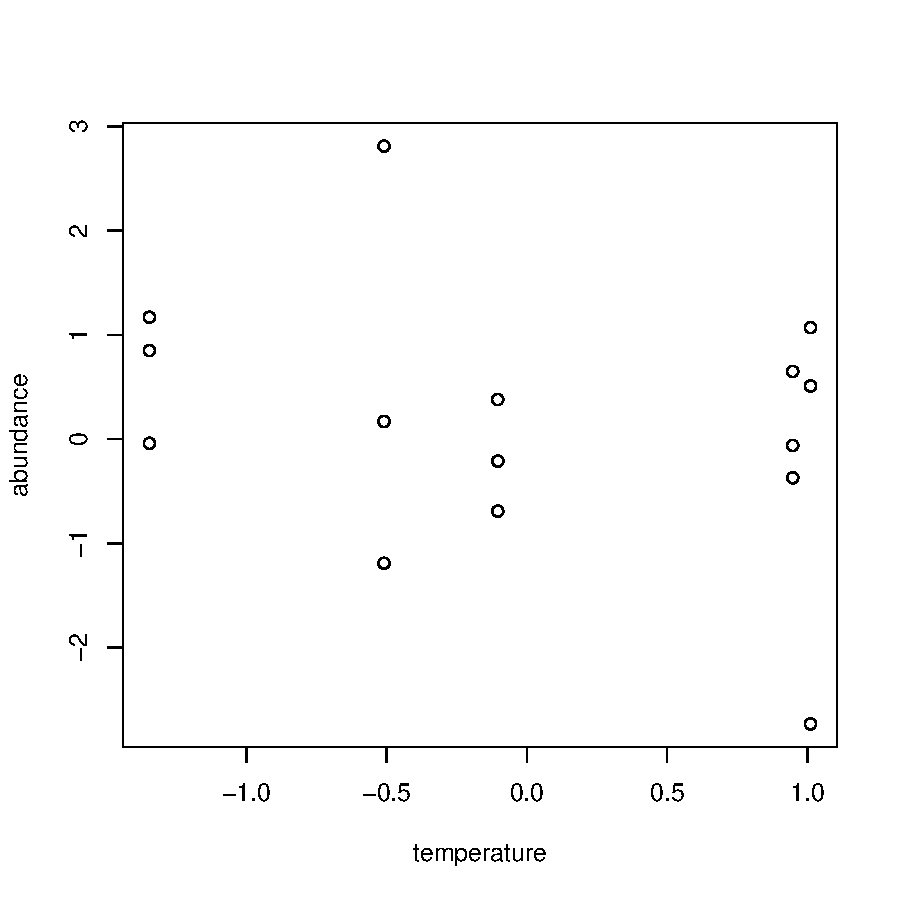
\includegraphics{sweave-015}
\end{frame}
\end{comment}%%%

\subsection[Coercion]{Coercing data lists to data frames}
\frame{\tableofcontents[currentsection,currentsubsection]}

\begin{frame}[fragile]
\begin{Schunk}
\begin{Sinput}
> as.data.frame(dl)
\end{Sinput}
\begin{Soutput}
   abundance temperature bodysize
1       1.17  -1.3453605    -0.45
2       0.65   0.9475797    -0.45
3       0.51   1.0109206    -0.45
4      -1.19  -0.5092608    -0.45
5      -0.69  -0.1038791    -0.45
6      -0.04  -1.3453605    -0.07
7      -0.06   0.9475797    -0.07
8      -2.73   1.0109206    -0.07
9       2.81  -0.5092608    -0.07
10     -0.21  -0.1038791    -0.07
11      0.85  -1.3453605     1.48
12     -0.37   0.9475797     1.48
13      1.07   1.0109206     1.48
14      0.17  -0.5092608     1.48
15      0.38  -0.1038791     1.48
\end{Soutput}
\end{Schunk}
\end{frame}

\begin{comment}%%
\begin{frame}[fragile]
\begin{Schunk}
\begin{Sinput}
> variablize(dl)
\end{Sinput}
\begin{Soutput}
      abundance.sppA abundance.sppB abundance.sppC temperature
siteA           1.17          -0.04           0.85  -1.3453605
siteB           0.65          -0.06          -0.37   0.9475797
siteC           0.51          -2.73           1.07   1.0109206
siteD          -1.19           2.81           0.17  -0.5092608
siteE          -0.69          -0.21           0.38  -0.1038791
\end{Soutput}
\end{Schunk}
\end{frame}

\begin{frame}[fragile]
\begin{Schunk}
\begin{Sinput}
> variablize(aperm(dl, c(2, 1)))
\end{Sinput}
\begin{Soutput}
     abundance.siteA abundance.siteB abundance.siteC abundance.siteD abundance.siteE bodysize
sppA            1.17            0.65            0.51           -1.19           -0.69    -0.45
sppB           -0.04           -0.06           -2.73            2.81           -0.21    -0.07
sppC            0.85           -0.37            1.07            0.17            0.38     1.48
\end{Soutput}
\end{Schunk}
\end{frame}
\end{comment}%%%

\subsection[Real data]{Real complex zooplankton community data}
\frame{\tableofcontents[currentsection,currentsubsection]}

\begin{frame}
\begin{center}
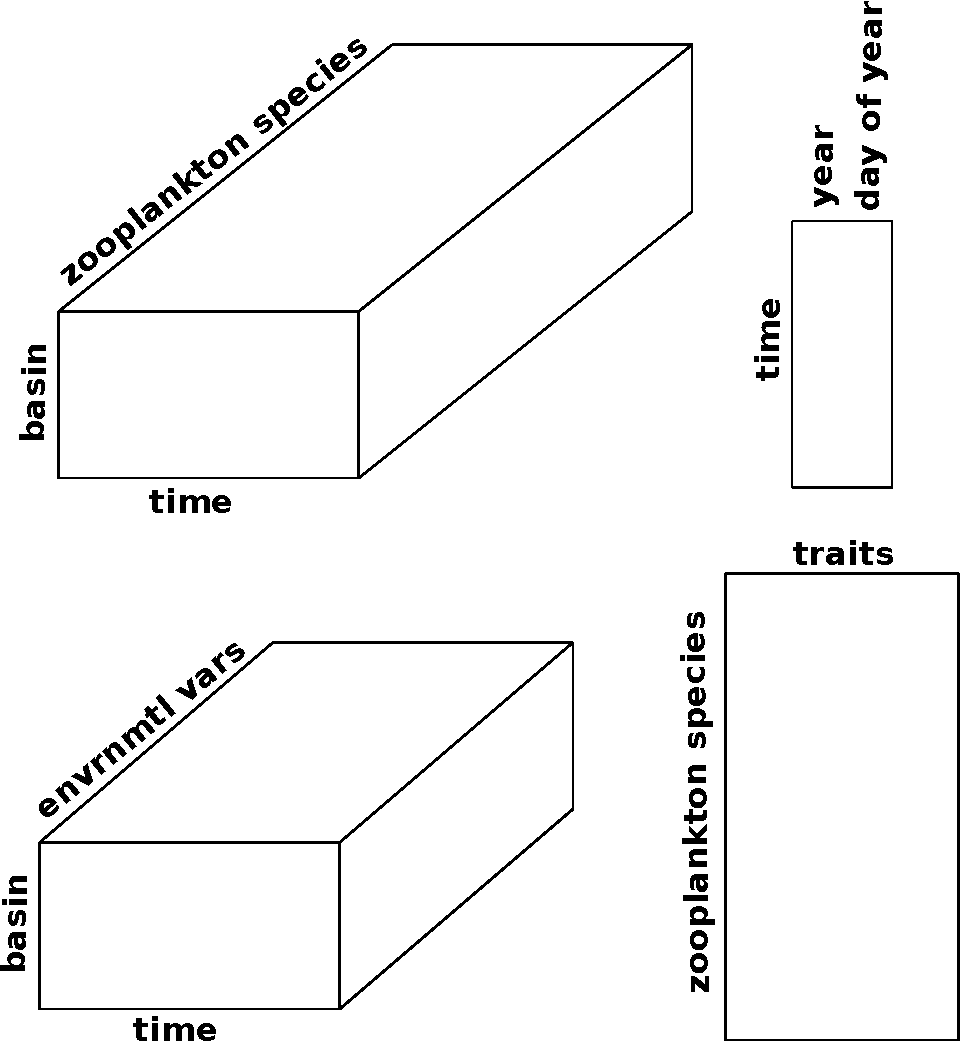
\includegraphics[width=6.5cm]{BeatrixTableCartoon}
\end{center}
\flushleft{Cantin et al. 2011 -- Lac Croche, Qu\'{e}bec, Canada}
\end{frame}

\begin{comment}%%%
\begin{frame}[fragile]
\begin{Schunk}
\begin{Sinput}
> dl <- data.list(Abundance = Y, X, W, Z, 
+ dnames = c("time", "species", "basin"))
\end{Sinput}
\end{Schunk}
\end{frame}
\end{comment}%%%

\begin{comment}
\begin{frame}[fragile]
\begin{tiny}
\begin{Schunk}
\begin{Sinput}
> summary(dl)
\end{Sinput}
\begin{Soutput}
$dims
        Abundance Temp.CV..Fluoro. Chl.CV..Fluoro. MaxTemp..Fl. MaxChl..Fl. Depth.TempMax.Fl.
time         TRUE             TRUE            TRUE         TRUE        TRUE              TRUE
species      TRUE            FALSE           FALSE        FALSE       FALSE             FALSE
basin        TRUE             TRUE            TRUE         TRUE        TRUE              TRUE
        DepthChlMax..Fl. Thermocline.Depth  Year  Week Habitat TrophicGroup FeedingType Length
time                TRUE              TRUE  TRUE  TRUE   FALSE        FALSE       FALSE  FALSE
species            FALSE             FALSE FALSE FALSE    TRUE         TRUE        TRUE   TRUE
basin               TRUE              TRUE FALSE FALSE   FALSE        FALSE       FALSE  FALSE
        Predator.protection.
time                   FALSE
species                 TRUE
basin                  FALSE
\end{Soutput}
\end{Schunk}
\end{tiny}
\end{frame}

\begin{frame}[fragile]
\begin{tiny}
\begin{Schunk}
\begin{Sinput}
> str(dl)
\end{Sinput}
\begin{Soutput}
List of 15
 $ Abundance           : num [1:16, 1:12, 1:3] 0.00134 0.00269 0.00361 0.00134 0.00226 ...
 $ Temp.CV..Fluoro.    : num [1:16, 1:3] 0.56 0.52 0.42 0.39 0.41 0.57 0.48 0.48 0.44 0.4 ...
 $ Chl.CV..Fluoro.     : num [1:16, 1:3] 0.92 0.94 1.04 1.05 0.82 0.92 0.79 0.79 0.27 0.27 ...
 $ MaxTemp..Fl.        : num [1:16, 1:3] 23.8 21.1 22.9 26.5 22.8 ...
 $ MaxChl..Fl.         : num [1:16, 1:3] 5.49 4.86 6.21 6.94 7.07 6.82 3.58 6.7 2.43 1.84 ...
 $ Depth.TempMax.Fl.   : num [1:16, 1:3] 0 1 2 0 1 1 0 1 1 0 ...
 $ DepthChlMax..Fl.    : num [1:16, 1:3] 5 4 7 6 5 8 5 6 5 5 ...
 $ Thermocline.Depth   : num [1:16, 1:3] 4.5 4.5 4.5 4.5 4.5 4.5 3.5 3.5 4 4.5 ...
 $ Year                : int [1:16(1d)] 2007 2007 2007 2007 2007 2007 2008 2008 2008 2008 ...
 $ Week                : int [1:16(1d)] 171 185 199 213 227 241 178 188 205 219 ...
 $ Habitat             : factor [1:12(1d)] Pelagic Pelagic Pelagic Pelagic ...
 $ TrophicGroup        : factor [1:12(1d)] Herbivore Herbivore Herbivore Herbivore ...
 $ FeedingType         : factor [1:12(1d)] D-filtration D-filtration B-filtration S-filtration ...
 $ Length              : num [1:12(1d)] 0.96 0.8 0.33 0.77 0.75 1.23 0.18 1.31 0.45 0.36 ...
 $ Predator.protection.: factor [1:12(1d)] N Y N Y ...
\end{Soutput}
\end{Schunk}
\end{tiny}
\end{frame}
\end{comment}%%

\begin{frame}[fragile]
\begin{Schunk}
\begin{Sinput}
> xyplot(Abundance ~ Chl.CV..Fluoro. | Length, 
+ data = as.data.frame(dl))
\end{Sinput}
\end{Schunk}
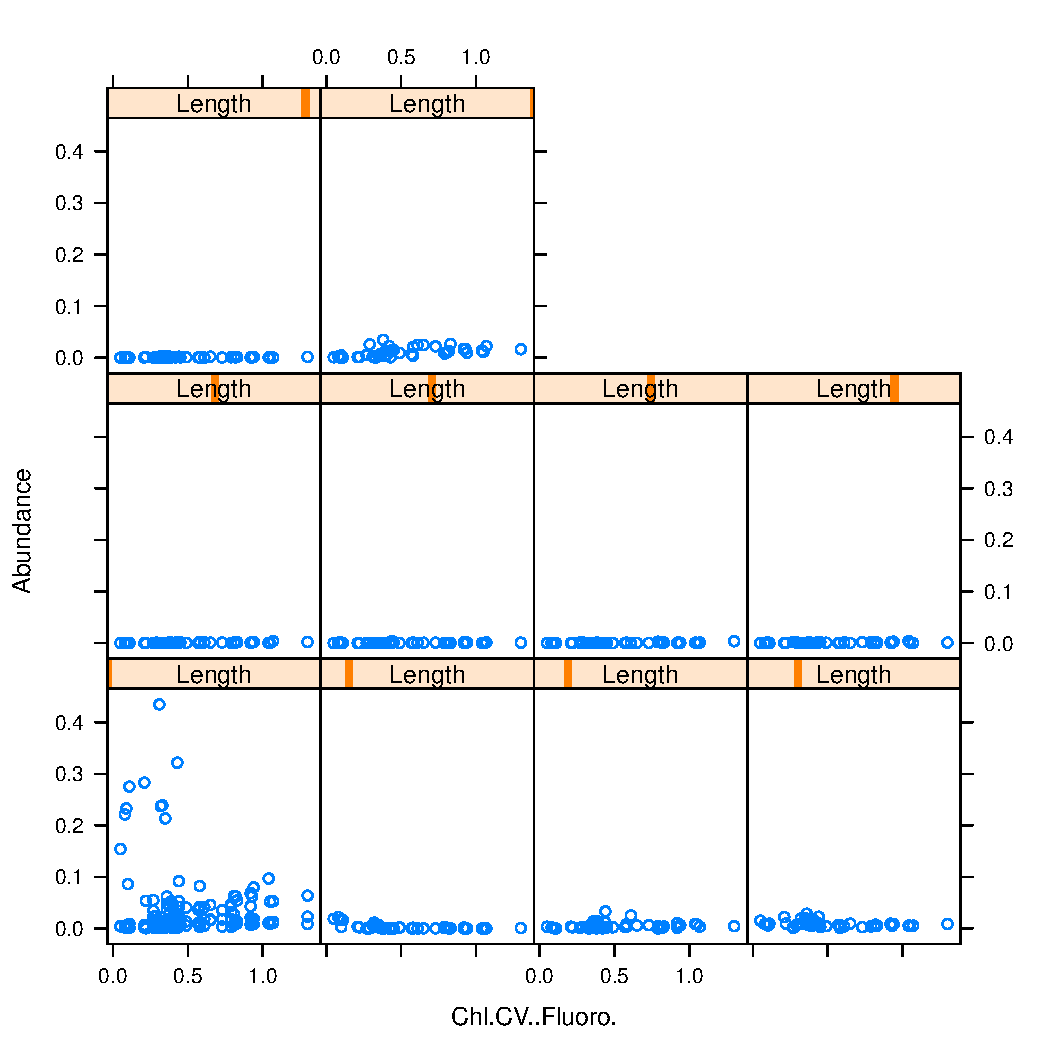
\includegraphics{sweave-026}
\end{frame}

\section{Conclusion}
\frame{\tableofcontents[currentsection]}

\begin{frame}
\begin{center}
\begin{block}{Take-home message}
Don't be scared of multiple table data sets.  \pause Collect more of them! \pause With the right data management framework, \pause multiple table data can be modeled in much the same way that we model single table data.
\end{block}
\end{center}
\end{frame}

\begin{comment}

%%%%%
\begin{frame}
\frametitle{Traits et phylog\'{e}nies}
\begin{center}
\includegraphics[width=4cm]{phylogeny}
\end{center}
\footnotesize{Cavender-Bares et al. (2009)}
\end{frame}
%%%%%

%%%%%
\begin{frame}
\frametitle{Tests d'hypoth\`{e}se}
\begin{center}
\includegraphics[width=6cm]{pillar}
\end{center}
\vspace{-0.5cm}
\footnotesize{Pillar and Duarte (2010)}
\end{frame}
%%%%%

%%%%%
\begin{frame}
\frametitle{Rarement utilis\'{e}s pour pr\'{e}dire}
\begin{center}
\includegraphics[width=6cm]{Ives}
\end{center}
\vspace{-0.5cm}
\footnotesize{Ives and Godrey (2006)}
\end{frame}
%%%%%

\subsection{Exemple illustratif}
\frame{\tableofcontents[currentsection,currentsubsection]}

\begin{frame}
\frametitle{Quatri\`{e}me coin}
\small
% latex table generated in R 2.10.1 by xtable 1.5-6 package
% Tue Feb  8 08:19:58 2011
\begin{table}[ht]
\begin{center}
\begin{tabular}{r|rrrr|r|}
  & sp 1 & sp 2 & sp 3 & sp 4 \\ 
  \hline
site 1 & 0.1 & 2.1 & 0.1 & 1.5  \\ 
  site 2 & 0.7 & -0.9 & 1.8 & 3.7  \\ 
  site 3 & 1.1 & 0.5 & 1.5 & 2.8  \\ 
  site 4 & 1.3 & -2.0 & 3.0 & -0.2  \\ 
  site 5 & 1.7 & 2.0 & 1.3 & 1.2  \\ 
  site 6 & 0.8 & -0.1 & 2.0 & 1.1  \\ 
  site 7 & -2.6 & -1.4 & 1.8 & 4.1  \\ 
  site 8 & -0.0 & 1.5 & 2.3 & 2.3  \\ 
   \hline
\end{tabular}
\end{center}
\end{table}\normalsize
\end{frame}

\begin{frame}
\frametitle{Quatri\`{e}me coin}
\small
% latex table generated in R 2.10.1 by xtable 1.5-6 package
% Tue Feb  8 08:19:58 2011
\begin{table}[ht]
\begin{center}
\begin{tabular}{r|rrrr|r|}
  & sp 1 & sp 2 & sp 3 & sp 4 & environment \\ 
  \hline
site 1 & 0.1 & 2.1 & 0.1 & 1.5 & -0.3 \\ 
  site 2 & 0.7 & -0.9 & 1.8 & 3.7 & 1.4 \\ 
  site 3 & 1.1 & 0.5 & 1.5 & 2.8 & -0.1 \\ 
  site 4 & 1.3 & -2.0 & 3.0 & -0.2 & 0.4 \\ 
  site 5 & 1.7 & 2.0 & 1.3 & 1.2 & -0.3 \\ 
  site 6 & 0.8 & -0.1 & 2.0 & 1.1 & -0.6 \\ 
  site 7 & -2.6 & -1.4 & 1.8 & 4.1 & 2.0 \\ 
  site 8 & -0.0 & 1.5 & 2.3 & 2.3 & 0.7 \\ 
   \hline
\end{tabular}
\end{center}
\end{table}\normalsize
\end{frame}

\begin{frame}
\frametitle{Quatri\`{e}me coin}
\small
% latex table generated in R 2.10.1 by xtable 1.5-6 package
% Tue Feb  8 08:19:58 2011
\begin{table}[ht]
\begin{center}
\begin{tabular}{r|rrrr|r|}
  & sp 1 & sp 2 & sp 3 & sp 4 & environment \\ 
  \hline
site 1 & 0.1 & 2.1 & 0.1 & 1.5 & -0.3 \\ 
  site 2 & 0.7 & -0.9 & 1.8 & 3.7 & 1.4 \\ 
  site 3 & 1.1 & 0.5 & 1.5 & 2.8 & -0.1 \\ 
  site 4 & 1.3 & -2.0 & 3.0 & -0.2 & 0.4 \\ 
  site 5 & 1.7 & 2.0 & 1.3 & 1.2 & -0.3 \\ 
  site 6 & 0.8 & -0.1 & 2.0 & 1.1 & -0.6 \\ 
  site 7 & -2.6 & -1.4 & 1.8 & 4.1 & 2.0 \\ 
  site 8 & -0.0 & 1.5 & 2.3 & 2.3 & 0.7 \\ 
   \hline
  trait & -1.0 & -1.0 & 1.0 & 1.0 & 0.8 \\ 
   \hline
\end{tabular}
\end{center}
\end{table}\normalsize 
\end{frame}

\begin{frame}
\frametitle{Quatri\`{e}me coin}
\small
% latex table generated in R 2.10.1 by xtable 1.5-6 package
% Tue Feb  8 08:19:58 2011
\begin{table}[ht]
\begin{center}
\begin{tabular}{r|rrrr|r|}
  & sp 1 & sp 2 & sp 3 & sp 4 & environment \\ 
  \hline
site 1 & 0.1 & 2.1 & 0.1 & 1.5 & -0.3 \\ 
  site 2 & 0.7 & -0.9 & 1.8 & 3.7 & 1.4 \\ 
  site 3 & 1.1 & 0.5 & 1.5 & 2.8 & -0.1 \\ 
  site 4 & 1.3 & -2.0 & 3.0 & -0.2 & 0.4 \\ 
  site 5 & 1.7 & 2.0 & 1.3 & 1.2 & -0.3 \\ 
  site 6 & 0.8 & -0.1 & 2.0 & 1.1 & -0.6 \\ 
  site 7 & -2.6 & -1.4 & 1.8 & 4.1 & 2.0 \\ 
  site 8 & -0.0 & 1.5 & 2.3 & 2.3 & 0.7 \\ 
   \hline
  trait & -1.0 & -1.0 & 1.0 & 1.0 & 0.8 \\ 
   \hline
\end{tabular}
\end{center}
\end{table}\normalsize 
\begin{textblock}{100}(10.2,-0.5)
$\uparrow$
\end{textblock}
\begin{textblock}{100}(11,-1.25)
$\leftarrow$
\end{textblock}
\begin{textblock}{100}(9.3,-1.25)
$\rightarrow$
\end{textblock}
\end{frame}

\begin{frame}
\frametitle{Quatri\`{e}me coin}
\small
% latex table generated in R 2.10.1 by xtable 1.5-6 package
% Tue Feb  8 08:19:58 2011
\begin{table}[ht]
\begin{center}
\begin{tabular}{r|rrrr|rr|}
  & sp 1 & sp 2 & sp 3 & sp 4 & intercept & environment \\ 
  \hline
site 1 & 0.1 & 2.1 & 0.1 & 1.5 & 1.0 & -0.3 \\ 
  site 2 & 0.7 & -0.9 & 1.8 & 3.7 & 1.0 & 1.4 \\ 
  site 3 & 1.1 & 0.5 & 1.5 & 2.8 & 1.0 & -0.1 \\ 
  site 4 & 1.3 & -2.0 & 3.0 & -0.2 & 1.0 & 0.4 \\ 
  site 5 & 1.7 & 2.0 & 1.3 & 1.2 & 1.0 & -0.3 \\ 
  site 6 & 0.8 & -0.1 & 2.0 & 1.1 & 1.0 & -0.6 \\ 
  site 7 & -2.6 & -1.4 & 1.8 & 4.1 & 1.0 & 2.0 \\ 
  site 8 & -0.0 & 1.5 & 2.3 & 2.3 & 1.0 & 0.7 \\ 
   \hline
intercept & 1.0 & 1.0 & 1.0 & 1.0 & 1.2 & -0.2 \\ 
  trait & -1.0 & -1.0 & 1.0 & 1.0 & 0.5 & 0.8 \\ 
   \hline
\end{tabular}
\end{center}
\end{table}\normalsize
\end{frame}


\begin{frame}
\begin{center}
\begin{figure}
\includegraphics{bilinear-005}
\end{figure}
\end{center}
\end{frame}

\begin{frame}[fragile]
\begin{center}
\begin{Schunk}
\begin{Soutput}
            intercept trait
intercept        1.15  0.46
environment     -0.15  0.84
\end{Soutput}
\end{Schunk}
\begin{figure}
\includegraphics{bilinear-007}
\end{figure}
\end{center}
\end{frame}

\section{Mod\`{e}les bilin\'{e}aires}

\subsection[Quatri\`{e}me coin]{Solution bilin\'{e}aire au probl\`{e}me du quatri\`{e}me coin}
\frame{\tableofcontents[currentsection,currentsubsection]}

\begin{frame}
\frametitle{Quatri\`{e}me coin}
\small
% latex table generated in R 2.10.1 by xtable 1.5-6 package
% Tue Feb  8 08:19:58 2011
\begin{table}[ht]
\begin{center}
\begin{tabular}{r|rrrr|rr|}
  & sp 1 & sp 2 & sp 3 & sp 4 & intercept & environment \\ 
  \hline
site 1 & 0.1 & 2.1 & 0.1 & 1.5 & 1.0 & -0.3 \\ 
  site 2 & 0.7 & -0.9 & 1.8 & 3.7 & 1.0 & 1.4 \\ 
  site 3 & 1.1 & 0.5 & 1.5 & 2.8 & 1.0 & -0.1 \\ 
  site 4 & 1.3 & -2.0 & 3.0 & -0.2 & 1.0 & 0.4 \\ 
  site 5 & 1.7 & 2.0 & 1.3 & 1.2 & 1.0 & -0.3 \\ 
  site 6 & 0.8 & -0.1 & 2.0 & 1.1 & 1.0 & -0.6 \\ 
  site 7 & -2.6 & -1.4 & 1.8 & 4.1 & 1.0 & 2.0 \\ 
  site 8 & -0.0 & 1.5 & 2.3 & 2.3 & 1.0 & 0.7 \\ 
   \hline
intercept & 1.0 & 1.0 & 1.0 & 1.0 & 1.2 & -0.2 \\ 
  trait & -1.0 & -1.0 & 1.0 & 1.0 & 0.5 & 0.8 \\ 
   \hline
\end{tabular}
\end{center}
\end{table}\normalsize
\end{frame}

\begin{frame}
\frametitle{Quatri\`{e}me coin}
\begin{center}
\includegraphics[width=5cm]{fourthcornerfigure.pdf}
\end{center}
\end{frame}

\begin{frame}
\begin{block}{D\'{e}finitions}
Variables: $y$ (communaut\'{e}), $x$ (environnement), $z$ (les traits) \\
\pause
Indices: $i$ (site), $j$ (esp\`{e}ces), $k$ (var. env.), $l$ (trait)
\pause
\end{block}
\begin{block}{Mod\`{e}le lin\'{e}aire}
\begin{equation}
\begin{gathered}
y_{ij} = \sum_{k=1}^{p} x_{ik}b_{kj} + e_{ij} \\
%\mathbf{Y} = \mathbf{XB} + \mathbf{E}
%\pause
\end{gathered}
\end{equation}
\end{block}
\pause
\begin{block}{Mod\`{e}le bilin\'{e}aire}
\begin{equation}
\begin{gathered}
y_{ij} = \sum_{k=1}^{p} \sum_{l=1}^{q} x_{ik}z_{jl}c_{kl} + e_{ij} \\
%\pause
%\mathbf{Y} = \mathbf{XCZ^{T}} + \mathbf{E}
\end{gathered}
\end{equation}
\end{block}
\end{frame}

\begin{frame}
\begin{center}
\begin{block}{Qu'est-ce que tout cela signifie?}
\begin{itemize}
\item Les mod\`{e}les bilin\'{e}aires ont une meilleure puissance statistique que les mod\`{e}les lin\'{e}aires multivari\'{e}s ``classique".
\pause
\begin{enumerate}
\item Les esp\`{e}ces agissent telles des r\'{e}plicats pour \'{e}tudier l'effet des traits \emph{et} % agissent telles = act like / act as
\pause
\item les sites agissent tels des r\'{e}plicats pour \'{e}tudier l'effet de l'environnement.
\pause
\item Pour les mod\`{e}les lin\'{e}aires classique, seulment les sites sont utilis\'{e}s comme r\'{e}plicats.
\end{enumerate}
\pause
\item Pas de param\`{e}tres repr\'{e}sentant chaque esp\`{e}ce mais seulment pour repr\'{e}senter les traits: les mod\`{e}les bilin\'{e}aires sont plus parcimonieux quand il y a moins de traits que d'esp\`{e}ces.
\pause
\item Quel est le prix \`{a} payer?  \pause  Les mod\`{e}les sont plus difficile \`{a} specifier (par exemple, quels traits doivent \^{e}tre utilis\'{e}s?)
\end{itemize}
\end{block}
\end{center}
\end{frame}

\subsection{Alg\`{e}bre bilin\'{e}aire 101}
\frame{\tableofcontents[currentsection,currentsubsection]}

\begin{frame}
\frametitle{Alg\`{e}bre bilin\'{e}aire 101}
\begin{itemize}
\item Alg\`{e}bre bilin\'{e}aire est une extension de l'alg\`{e}bre lin\'{e}aire
\pause
\item L'alg\`{e}bre bilin\'{e}aire traite les matrices comme l'alg\`{e}bre lin\'{e}aire traiterait les vecteurs %%% pick up from here.
\pause
\item Cependent, ces deux domaines sont connexes
\pause
\item Il est possible de transformer une repr\'{e}sentation bilin\'{e}aire en une repr\'{e}sentation lin\'{e}aires
\pause
\item Deux op\'{e}rations math\'{e}matiques permettent cette transformation:  
\begin{enumerate}
\item l'op\'{e}rateur vec
\item le produit de Kronecker ($\otimes$)
\end{enumerate}
\end{itemize}
\end{frame}

\begin{frame}
\begin{block}{Comprendre l'op\'{e}rateur vec}
\begin{equation}
\mathbf{Y} = \left(
	\begin{array}{cccc}
		y_{11} & y_{12} & \ldots & y_{1m} \\
		y_{21} & y_{22} & \ldots & y_{2m} \\
		\vdots & \vdots & \ddots & \vdots \\
		y_{n1} & y_{n2} & \ldots & y_{nm}
	\end{array}
\right),\pause
\mathrm{vec}(\mathbf{Y}) = \left(
	\begin{array}{c}
		y_{11} \\
		y_{21} \\
		\vdots \\
		y_{n1} \\
		\hline
		y_{12} \\
		y_{22} \\
		\vdots \\
		y_{n2} \\
		\hline
		\vdots \\
		\hline
		y_{1m} \\
		y_{2m} \\
		\vdots \\
		y_{nm}
	\end{array}
\right)
\end{equation}
\end{block}
\end{frame}

\begin{frame}
\begin{block}{Comprendre le produit de Kronecker}
\tiny
\begin{equation}
\begin{gathered}
\mathbf{Z}\otimes\mathbf{X} = \\
\begin{bmatrix}
   z_{11} x_{11} & z_{11} x_{12} & \cdots & z_{11} x_{1p} & 
                   \cdots & \cdots & z_{1q} x_{11} & z_{1q} x_{12} & \cdots & z_{1q} x_{1p} \\
   z_{11} x_{21} & z_{11} x_{22} & \cdots & z_{11} x_{2p} & 
                   \cdots & \cdots & z_{1q} x_{21} & z_{1q} x_{22} & \cdots & z_{1q} x_{2p} \\
   \vdots & \vdots & \ddots & \vdots & & & \vdots & \vdots & \ddots & \vdots \\
   z_{11} x_{n1} & z_{11} x_{n2} & \cdots & z_{11} x_{np} & 
                   \cdots & \cdots & z_{1q} x_{n1} & z_{1q} x_{n2} & \cdots & z_{1q} x_{np} \\
   \vdots & \vdots & & \vdots & \ddots & & \vdots & \vdots & & \vdots \\
   \vdots & \vdots & & \vdots & & \ddots & \vdots & \vdots & & \vdots \\
   z_{m1} x_{11} & z_{m1} x_{12} & \cdots & z_{m1} x_{1p} & 
                   \cdots & \cdots & z_{mq} x_{11} & z_{mq} x_{12} & \cdots & z_{mq} x_{1p} \\
   z_{m1} x_{21} & z_{m1} x_{22} & \cdots & z_{m1} x_{2p} & 
                   \cdots & \cdots & z_{mq} x_{21} & z_{mq} x_{22} & \cdots & z_{mq} x_{2p} \\
   \vdots & \vdots & \ddots & \vdots & & & \vdots & \vdots & \ddots & \vdots \\
   z_{m1} x_{n1} & z_{m1} x_{n2} & \cdots & z_{m1} x_{np} & 
                   \cdots & \cdots & z_{mq} x_{n1} & z_{mq} x_{n2} & \cdots & z_{mq} x_{np} 
\end{bmatrix}
\end{gathered}
\end{equation}
\normalsize
\end{block}
\end{frame}

\subsection{Un exemple pratique}
\frame{\tableofcontents[currentsection,currentsubsection]}

\begin{frame}
\begin{block}{Les communaut\'{e}s d'oiseaux (Dol\'{e}dec et al. 1996)}
\begin{itemize}
\item 51 sites
\item 40 esp\`{e}ces
\item 11 variables environnementales
\item 4 traits d'esp\`{e}ces
\end{itemize}
\end{block}
\pause
\begin{block}{Mod\`{e}les bilin\'{e}aires logistiques}
\begin{equation}
\mathrm{logit}(\mu_{ij}) = \sum_{k=1}^{p} \sum_{l=1}^{q} x_{ik}c_{kl}z_{jl}
\end{equation}
\end{block}
\end{frame}

\begin{frame}
\frametitle{Quatri\`{e}me coin}
\includegraphics{bilinear-024}
\end{frame}

\begin{frame}
\begin{center}
\frametitle{Valeurs ajust\'{e}es}
\vspace{-0.5cm}
\includegraphics[width=8.5cm]{fittedvalues}
\end{center}
\end{frame}

\section{Conclusion}
\frame{\tableofcontents[currentsection,currentsubsection]}

\begin{frame}
\begin{center}
\begin{block}{Avantages des mod\`{e}les bilin\'{e}aires}
\begin{enumerate}
\item Facilement interpr\'{e}tables (le quatri\`{e}me coin)
\pause
\item Facilement utilisables pour faire des pr\'{e}dictions
\pause
\item Il s'agit simplement de mod\'{e}lisation lin\'{e}aire avec interactions!
\pause
\item Plus parcimonieux que les mod\`{e}les multivari\'{e}s classiques.
\end{enumerate}
\end{block}
\end{center}
\end{frame}

\begin{frame}
\begin{center}
\begin{block}{D\'{e}fi des mod\`{e}les bilin\'{e}aires}
\begin{enumerate}
\item La definition du mod\`{e}le n\'{e}cessite plus de r\'{e}flexion
\pause 
\item Les interactions peuvent \^{e}tre difficiles \`{a} interpr\'{e}ter si le mod\`{e}le n'est pas correctement d\'{e}fini au d\'{e}part
\end{enumerate}
\end{block}
\end{center}
\end{frame}

\end{comment}

\section{}

\begin{frame}
\begin{center}
\frametitle{Acknowledgements}
\vspace{-1cm}
\begin{itemize}
\item Natural Sciences and Engineering Research Council of Canada
\item Laura Timms (McGill University)
\item Beatrix Beisner (Universit\'{e} du Qu\'{e}bec \`{a} Montr\'{e}al)
\item Ben Bolker (McMaster University)
\item The many people who gave their time to develop free software: \R\ and \LaTeX\
\end{itemize}
\end{center}
http://multitable.r-forge.r-project.org/ \\
\vspace{0.3cm}
\includegraphics[width=2cm]{multitablelogo}
\end{frame}



\end{document}
